\section{Reševanje enačb}
\label{pogl:enacbe}

V tem poglavju s prepogibanjem papirja rešujemo enačbe z racionalnimi koeficienti. Njihove rešitve bomo konstruirali v evklidski ravnini, ki jo predstavlja list papirja. Spomnimo se, da smo origami števila definirali kot vsa števila, ki jih lahko s prepogibanjem konstruiramo preko na začetku danega izhodišča $O$ in števila $1$ na realni osi (definicija~\ref{def:origami_stevilo}), evklidska ravnina pa je v bijekciji s kompleksno ravnino, dano v definiciji. Zaradi večje preglednosti bomo lahko pomožne pregibe in točke (ki bi jih sicer znali konstruirati z origamijem, npr.\ zrcaljene točke) narisali kar z ravnilom in pisalom.

Začnimo z najbolj osnovno, t.\ j.\ linearno enačbo. Enačba $ax + b = 0$, kjer $a, b \in \Q$ in $a \neq 0$ ima rešitev $x = -b/a$, ki je racionalno število, torej origami število in samo po sebi konstruktibilno. Če bi želeli rešitev konstruirati geometrijsko preko pregibov, v ravnini prepognemo premico $y = ax + b$ (napravimo pregib npr.\ skozi točki (0, b) in (1, a+b)) in njeno presečišče z abscisno osjo nam da iskano rešitev (slika~\ref{fig:lin_en}).

\begin{figure}[h]
    \centering
    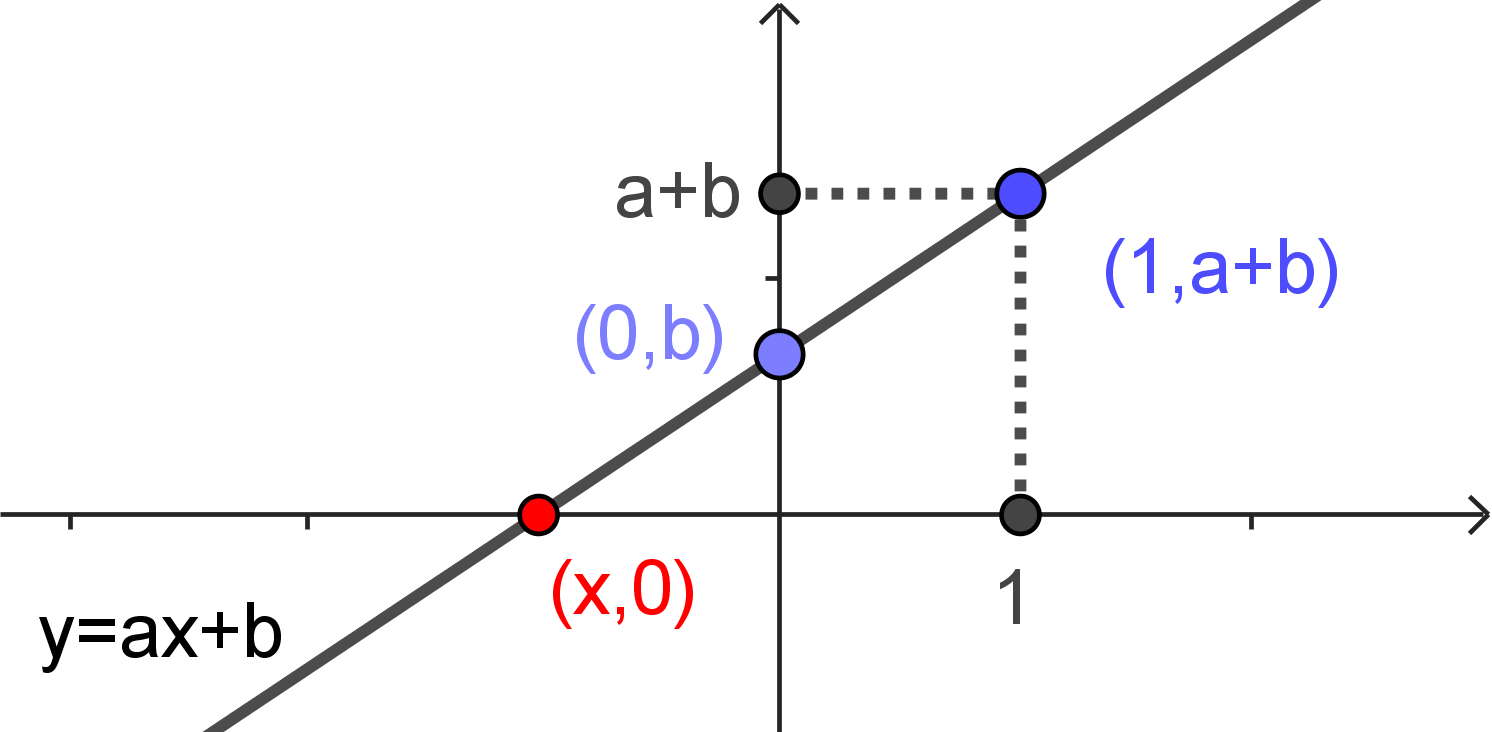
\includegraphics[width=0.5\textwidth]{images/linearna_enacba.png}
    \caption[Reševanje linearne enačbe]{Reševanje linearne enačbe $ax+b=0$. Abscisa rdeče točke je iskana rešitev.}
    \label{fig:lin_en}
\end{figure}

Uporaba origamija je za reševanje linearne enačbe očitno manj praktična kot računanje rešitve. Bolj zanimivo je reševanje kvadratne in kubične enačbe. Ker za njune rešitve obstajata splošni formuli, bi lahko rešitve najprej izračunali in nato preko operacij seštevanja, odštevanja, množenja, deljenja in korenjenja konstruirali s prepogibanjem, vendar je to časovno preveč potratno. Pogledali si bomo, kako se z origamijem lahko temu izognemo in rešitev konstruiramo brez uporabe računskih operacij.

Ključno vlogo bosta v nadaljevanju odigrali origami operaciji~\ref{op:O6} in~\ref{op:O7}. Prva nam hkrati s konstrukcijo tangente na parabolo določi tudi točko na paraboli, skozi katero je pregib tangenten na stožnico, to pa je ekvivalentno reševanju kvadratne enačbe. Druga s konstrukcijo skupne tangente na dve paraboli omogoča reševanje kubične enačbe -- to pokaže npr.\ Alperin v~\cite[str.\ 129]{alperin2000}, ko izpelje koeficient skupne tangente na dani paraboli, za katerega se izkaže, da je rešitev kubične enačbe. Število skupnih tangent je torej enako številu rešitev kubične enačbe, kar pomeni, da imata paraboli v evklidski ravnini največ tri skupne tangente.

V teoriji bi nam prepogibanje papirja pomagalo tudi pri reševanju kvartičnih enačb, saj zanje še obstaja splošna formula (vendar zaradi dolžine praktično neuporabna) in tudi vemo, da lahko enačbo četrte stopnje prevedemo na enačbe nižje stopnje (gl.\ \cite{wikiquartic}, \cite{quartics2012}). Geometrično pa je to reševanje potem težje izvedljivo in zato manj motivacijsko, saj bi postopek reševanja sistema dveh enačb zahteval veliko več pregibov kot pri reševanju le ene kubične ali kvadratne enačbe, pa tudi vmesne rezutate bi morali računati. Tako bi se lahko tu z reševanjem enačb preko origamija ustavili, vendar obstajajo alternativne rešitve. V~\cite{edwards2001} je opisan postopek, ki preko \textcolor{red}{projektivne geometrije in dualnih stožnic (malo preuredi izrazoslovje, če ni ok)} ter z Belochinim pregibom reši splošno kubično in nato tudi kvartično enačbo neke določene oblike. Postopek si bomo tudi sami pogledali, saj je zelo zanimiv iz vidika projektivne geometrije.

Za enačbe pete in višjih stopenj pa splošna formula za rešitve ne obstaja več (to vemo po \emph{Abel-Ruffinijev} izreku, gl.\ \cite{mrinal2019}). Kljub temu se da z origamijem še vedno konstruirati rešitve nekaterih enačb višjih stopenj, vendar ne obstaja postopek z enkratnimi prepogibi -- potrebno se je poslužiti dvojnih (\emph{two-fold}) ali večkratnih (\emph{multi-fold}) prepogibov (gl.\ poglavje~\ref{pogl:multifold}) \textcolor{red}{(če ga boš vključila)}.

\subsubsection*{Reševanje enačb s prevedbo ekvlidskih konstrukcij}

Z evklidskim orodjem lahko rešujemo enačbe druge stopnje, saj znamo konstruirati kvadratni koren poljubnega origami-konstruktibilnega števila. Ker vemo, da lahko s prepogibanjem papirja konstruiramo vse (in še več), kar se da z evklidskim orodjem, je včasih lažje za rešitev nekega problema najti (bolj domačo) evklidsko konstrukcijo, ki jo lahko nato preko origami operacij preobrazimo v origami konstrukcijo.

Kot primer tega Hull v~\cite[str.\ 38]{hull2020} navaja Lillovo konstrukcijo rešitve kvadratne enačbe preko krožnice -- na sliki~\ref{fig:par_primer_hull_lill} levo je prikaz evklidske kosntrukcije, desno pa prevedba na origami konstrukcijo. Lahek dokaz, zakaj deluje, je prepuščen bralcu.

\begin{figure}[h]
    \centering
    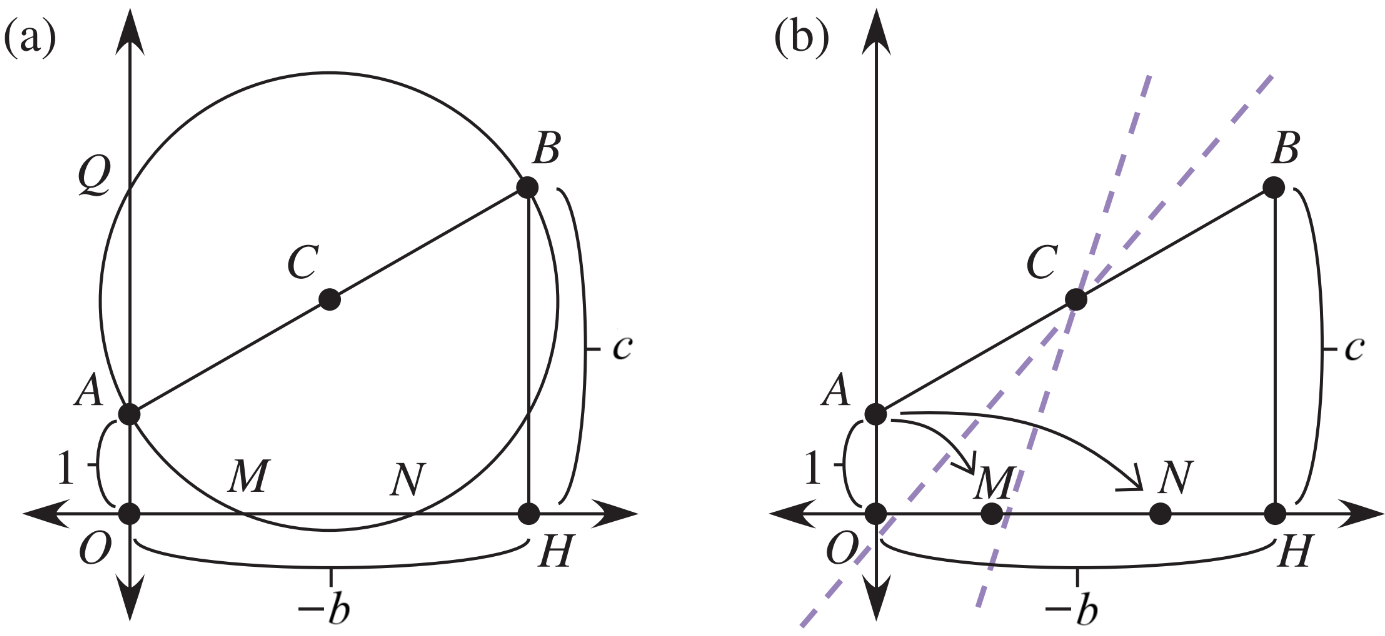
\includegraphics[width=0.7\textwidth]{images/kvadratna_enacba/primer_hull_lill.png}
    \caption[Primer reševanja kvadratne enačbe z evklidskim orodjem]{Reševanje enačbe $x^2 + ax + b = 0$. Vzeto iz~\cite[str.\ 38]{hull2020}.}
    \label{fig:par_primer_hull_lill}
\end{figure}

\subsection{Reševanje kvadratne enačbe preko tangente na parabolo}
\label{podpogl:kvadratna_enacba}

Rešujemo enačbo oblike
$$ a x^2 + b x + c = 0, $$
kjer so $a, b, c \in \Q$ in velja $a \neq 0$.  Njeni splošni rešitvi sta
$$ x_{1,2} = \frac{-b \pm \sqrt{b^2 - 4ac}}{2a}.$$

Postopek, ki si ga bomo pogledali v nadaljevanju, predpostavlja $a = 1$. Ker je vodilni koeficient neničeln, lahko z njim enačbo delimo in pri tem še vedno dobimo racionalne koeficiente, zato lahko predpostavko brez škode za splošnost sprejmemo. Nova oblika enačbe je tako
\begin{equation}
    \label{eq:spl_kv_en}
    x^2 + bx + c = 0.
\end{equation}
Predpostavimo, da ima enačba dve različni realni rešitvi oz.\ da je diskriminanta enačbe pozitivna, t.\ j.\ $D = b^2 - 4c > 0$. Če realnih ničel ni, o origami konstrukciji rešitev namreč nima smisla razpravljati. Če je rešitev ena, je podana kot $x = -b/2$, kar je origami-konstruktibilno število in se ga lahko takoj konstruira.

Enačba~\ref{eq:spl_kv_en} nam ob teh predpostavkah torej poda pokončno parabolo $y = x^2 + bx + c$ z vodoravno premico vodnico in dvema ničlama, ki sta rešitvi naše enačbe. Iščemo abscisi presečišč parabole z abscisno osjo.

Zopet se bomo poslužili dosedanjega znanja o operaciji~\ref{op:O6}. Ta nam s pregibom skozi dano točko $B$, ki točko $A$ položi na premico $a$, konstruira tangento na parabolo z goriščem v točki $A$ in premico vodnico $a$.

Naša parabola je z enačbo seveda natančno določena. Ideja iskane konstrukcije rešitev enačbe je določiti tako točko $B$ (najlažje kar na osi parabole), da bi nam izvedba operacije~\ref{op:O6} podala tangento na parabolo ravno v njeni ničli. Želeni pregib mora potekati skozi točko $B$ in gorišče $A$ položiti na tisto točko $A'$ na premici vodnici $a$, ki ima enako absciso kot ničla parabole. (gl.\ sliko~\ref{fig:tockaB_in_O6}). Taka točka $B$ je z osjo parabole in katerokoli izmed ničlama (zaradi simetrije) natanko določena.

\begin{figure}[h]
    \centering
    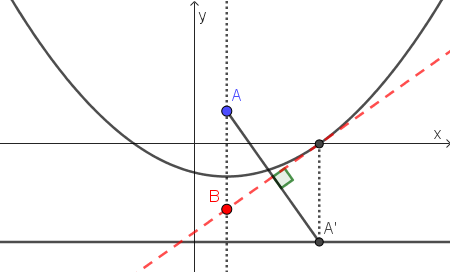
\includegraphics[width=0.5\textwidth]{images/kvadratna_enacba/tockaB_in_O6.png}
    \caption[Iskanje točke $B$]{Operacijo~\ref{op:O6} skozi iskano točko $B$ poda rešitev kvadratne enačbe.}
    \label{fig:tockaB_in_O6}
\end{figure}

Edina nevarnost, da ta konstrukcija ne bo delovala, je možnost, da točka $B$ kdaj ne bo origami-konstruktibilna točka. Zato sedaj izračunajmo njene koordinate in se prepričajmo, da se to nikoli ne bo zgodilo.

Najprej iz dane enačbe parabole določimo njeno gorišče $A$ in premico vodnico $a$. Spomnimo se, da iz enačbe oblike
$$ (x - x_0)^2 = 2p(y - y_0) $$
razberemo njeno teme $(x_0, y_0)$, gorišče $(x_0, y_0 + p/2)$ in enačbo premice vodnice $y = y_0 - p/2$. V našem primeru enačbo $y = x^2 + bx + c$ preoblikujemo v
$$ \left(x-\left(-\frac{b}{2}\right)\right)^2 = 2 \cdot \frac{1}{2} \left(y - \left(c - \frac{b^2}{4}\right)\right). $$
S tem sta gorišče $A$ in premica vodnica $a$ določena:
$$ A\left(-\frac{b}{2}, c - \frac{b^2}{4} + \frac{1}{4}\right) \text{ in } a: y = c - \frac{b^2}{4} - \frac{1}{4}. $$

Naj bo $t$ ena izmed rešitev enačbe~\ref{eq:spl_kv_en}. Na premici $a$ z $A'$ označimo točko z absciso $t$. Poiščimo enačbo pregiba, ki gorišče $A$ položi v točko $A'$. Ta pregib bo tangenten na parabolo ravno v njeni ničli, njegovo presečišče z osjo parabole $ x = -b/2 $ pa nam bo določilo točko $B$.

Koeficient nosilke daljice $AA'$ je $ - 1/(2t + b)$, torej je koeficient pregiba $k = 2t + b$. Pregib je po konstrukciji tangenten na parabolo v ničli $(t, 0)$, torej je njegova enačba
$$ y = (2t + b)(x - t) = (2t + b)x - 2t^2 - bt = (2t + b)x - t^2 + c. $$
Pri tem smo upoštevali, da velja $t^2 + bt + c = 0$. Presečišče pregiba in osi parabole je tako točka $B$ z absciso $ x = -b/2 $ in ordinato
$$ y = (2t + b)\left(-\frac{b}{2}\right) - t^2 + c = - t^2 - tb + c - \frac{b^2}{2} = c + c - \frac{b^2}{2} = 2c - \frac{b^2}{2}.$$
Obe koordinati sta racionalni, torej je točka $B$ konstruktibilna točka. Ker leži na osi parabole, nam poda obe rešitvi enačbe -- pregiba sta si simetrična glede na os. Povzemimo sedaj postopek konstrukcije rešitve kvadratne enačbe~\ref{eq:spl_kv_en}:
\begin{enumerate}
    \item V koordinatnem sistemu označimo gorišče $A\left(-\frac{b}{2}, c - \frac{b^2}{4} + \frac{1}{4}\right)$, premico vodnico $a: y = c - \frac{b^2}{4} - \frac{1}{4}$ in točko $B(-\frac{b}{2}, 2c - \frac{b^2}{2})$.
    \item Z operacijo~\ref{op:O6} naredimo pregib skozi točko $B$, ki točko $A$ položi na premico $a$ (če je diskriminanta enačbe pozitivna, sta možna pregiba dva).
    \item Skozi sliko točke $A$ naredimo vertikalen pregib in abscisa njegovega presečišča z abscisno osjo je ničla dane enačbe.
\end{enumerate}

\textbf{Primer:} Poiščimo rešitve enačbe $x^2 - x - 1 = 0$. Določimo obe točki in premico: $A(\frac{1}{2}, -1)$, $B(\frac{1}{2}, -\frac{5}{2})$ in $a: y = -\frac{3}{2}$ (na sliki~\ref{fig:par_primer_hull} so zaporedoma uporabljene oznake $P_1, P_2$ in $L$). Opravimo operacijo~\ref{op:O6} in označimo presečišče abscisne osi in pravokotnice nanjo skozi sliko točke $A$. Če smo bili pri pregibanju natančni, dobimo presečišči pri $x_{1,2} = \frac{1 \pm \sqrt{5}}{2}$.

\begin{figure}[h]
    \centering
    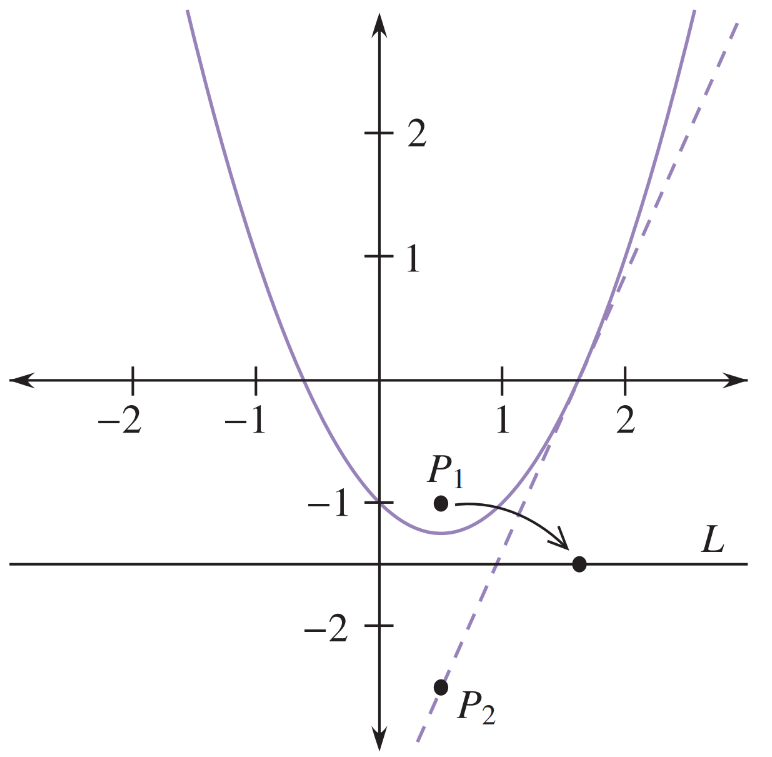
\includegraphics[width=0.4\textwidth]{images/kvadratna_enacba/primer_hull.png}
    \caption[Primer reševanja kvadratne enačbe]{Reševanje enačbe $x^2 - x - 1 = 0$ preko tangente na parabolo. Vzeto iz~\cite[str.\ 37]{hull2020}.}
    \label{fig:par_primer_hull}
\end{figure}

Metoda je enostavna, vendar v resnici zopet ne najbolj praktično izvedljiva, saj so lahko točki $A$ in $B$ ter premica $a$ težje origami-konstruktibilni. V naslednjem poglavju bomo med drugim spoznali Lillovo metodo, preko katere bomo z operacijo~\ref{op:O6} do rešitve prišli hitreje in enostavneje (gl.\ razdelek~\ref{podpodl:kvadr_en_lill}).

\subsection{Belochin postopek z Lillovo metodo}
\label{podpogl:kubicna_enacba}

Vzemimo enačbo oblike
$$ a x^3 + b x^2 + c x + d = 0, $$
kjer so $a, b, c, d \in \Q$ in velja $a \neq 0$. Tu je navedena ena oblika zapisa njene splošne rešitve:

\begin{align*}
    Q &= \sqrt{(2b^3 - 9abc + 27a^2d)^2 - 4(b^2 - 3ac)^3} \\
    C &= \sqrt[3]{\frac{1}{2}(Q + 2b^3 - 9abc + 27a^2d)} \\
    x_1 &= - \frac{b}{3a} - \frac{C}{3a} - \frac{b^2 - 3ac}{3aC} \\
    x_2 &= - \frac{b}{3a} + \frac{C(1 + i\sqrt{3})}{6a} + \frac{(1 - i\sqrt{3})(b^2 - 3ac)}{6aC} \\
    x_2 &= - \frac{b}{3a} + \frac{C(1 - i\sqrt{3})}{6a} + \frac{(1 + i\sqrt{3})(b^2 - 3ac)}{6aC}
\end{align*}

Operacija~\ref{op:O6} nam je preko konstrukcije tangente na parabolo pomagala rešiti kvadratno enačbo. Spomnimo se, da je Belocheva to v tridesetih letih prejšnjega stoletja nadgradila z operacijo~\ref{op:O7}, ki nam konstruira skupno tangento na dve paraboli, pregib pa imenujemo \emph{Belochin pregib}. Z njim je kot prva odkrila resnično moč origami konstrukcij, a je žal trajalo več kot pol stoletja, da so matematiki začeli ceniti njeno odkritje. Zgodilo se je celo, da so nekateri neodvisno od nje odkrili ta pregib in iznašli svoje postopke, ne da bi sploh poznali njeno delo.

Seznanili se bomo z Lillovo metodo, s katero lahko v teoriji rešimo enačbo poljubne stopnje. V središču naše pozornosti bo Belochin origami postopek za reševanje kubične enačbe, na koncu pa bomo Lillovo metodo uporabili tudi za reševanje kvadratne enačbe.

\subsubsection{Reševanje kubične enačbe z Belochinim postopkom}

Belocheva je sama odkrila naslednji postopek reševanja kubične enačbe, kjer nam vsak Belochin pregib poda eno izmed rešitev. Število teh pregibov pa je, kot smo premislili že v uvodu poglavja, enako številu rešitev dane enačbe. Postopek temelji na Lillovi genialni metode iskanja ničel poljubnih polinomov z realnimi koeficienti, ki si jo bomo v naslednjem razdelku podrobneje pogledali, avtorica pa je zaslužna za to, da se jo zelo enostavno konstruira tudi v praksi.

\subsubsection*{Lillova metoda}

Avstrijski inženir Eduard Lill je l.\ 1867 v svojem članku~\cite{lill1867} opisal inovativen postopek, ki je v svoji osnovi čisto enostaven. Imejmo poljuben polinom $ p(x) = a_n x^n + a_{n-1} x^{n-1} + \ldots + a_2 x^2 + a_1 x + a_0 $ z realnimi koeficienti in iščemo njegove realne ničle, če obstajajo. Lill je iz njegovih koeficientov v ravnini ustvaril enolično pot. 

Običajno pri opisovanju poteka konstrukcije uporabljamo figuro želve, katere pot nas zanima. Želva nam v vsakem trenutku kaže, kam je usmerjena in v katero smer se premika. Na začetku jo postavimo v koordinatno izhodišče $O$ tako, da gleda v pozitivno smer $x$-osi. Želva najprej v to smer prehodi razdaljo, enako koeficientu $a_n$. Nato se obrne za $90^\circ$ v pozitivno smer (nasprotno smer urinega kazalca) in prehodi naslednjo razdaljo $a_{n-1}$. To ponovi za vsak koeficient polinoma in po prehojeni razdalji $a_0$ se ustavi v neki točki $T$ (slika~\ref{fig:primera_zelve}). Če je kateri od koeficientov negativen, želva hodi ritensko (primer (b) na sliki~\ref{fig:primera_zelve} za koeficiente $a_3, a_2$ in $a_0$), v primeru ničelnega koeficienta pa obstoji na mestu in se samo obrne. S potjo želve dobimo lomljeno črto iz največ $n+1$ daljic, ki jih brez škode označujmo kar z njihovimi ``pripadajočimi'' koeficienti.

\begin{figure}[h]
    \centering
    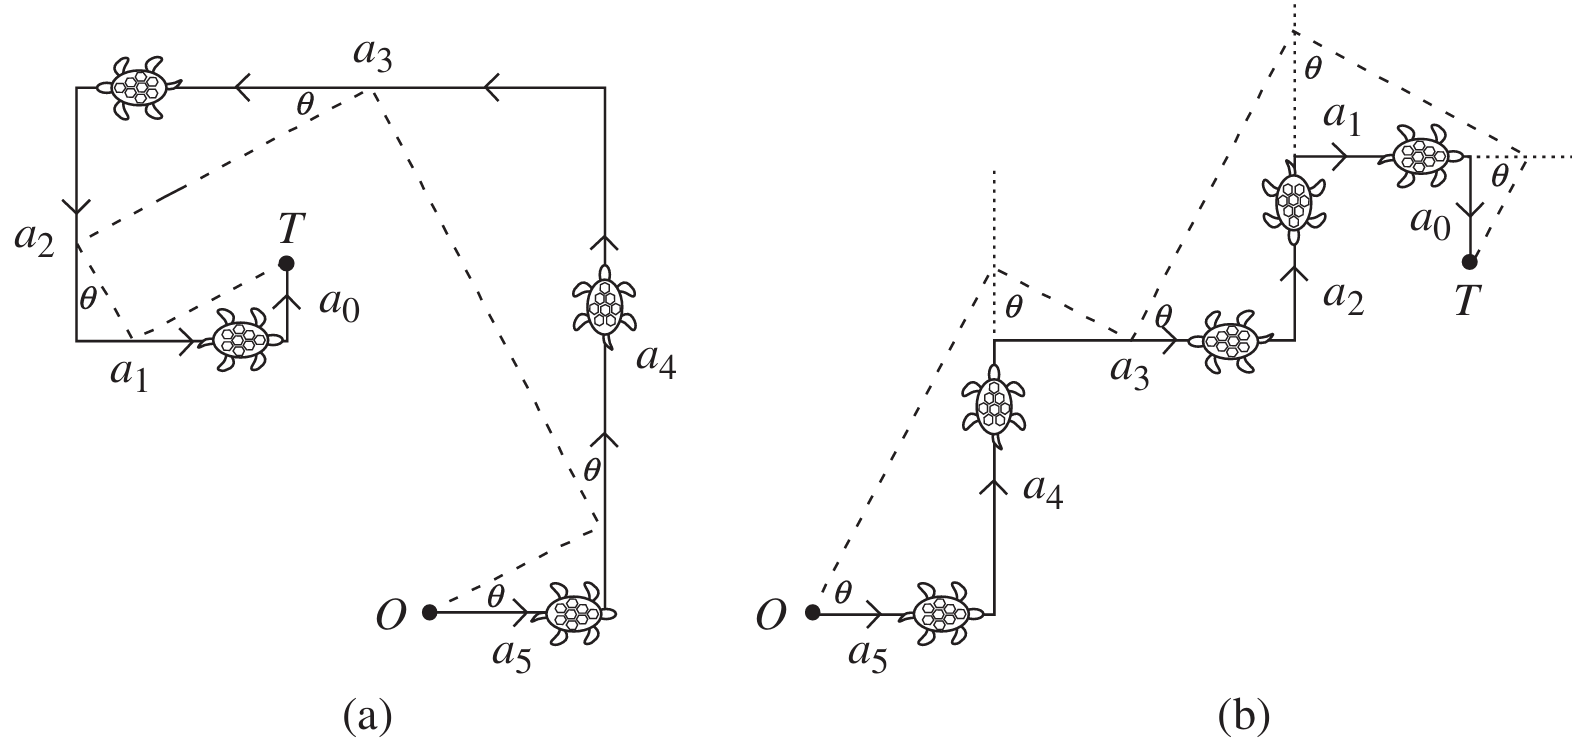
\includegraphics[width=0.9\textwidth]{images/kubična enačba/primera_zelvine_poti.png}
    \caption[Primera želvine poti]{Primera želvine poti za polinoma pete stopnje. Vzeto iz~\cite[str.\ 311]{hull2011}.}
    \label{fig:primera_zelve}
\end{figure}

Sedaj se v izhodišče $O$ postavimo še mi in z laserskim žarkom poskusimo zadeti želvo v točki $T$ tako, da žarek najprej usmerimo daljico $a_{n-1}$, od katere se odbije v daljico $a_{n-2}$, od te v daljico $a_{n-3}$ in tako naprej (slika~\ref{fig:primera_zelve}). Pri tem upoštevamo troje:
\begin{itemize}
    \item laserski žarek ne upošteva odbojnega zakona in se od daljice vedno odbije pod kotom $90^\circ$, zato so vpadni koti žarka na vse daljice med seboj enaki in prav tako to velja za odbojne kote;
    \item žarek se lahko odbije tudi od nosilke daljice;
    \item vsakič sta možni dve smeri odboja -- na isto ali drugo stran daljice oz.\ njene nosilke -- izberemo pa tisto, ki nam omogoči, da sploh lahko zadenemo naslednjo daljico.
\end{itemize}
Taka pot žarka vedno obstaja in je enolična. Vpadni kot, ki ga v točki $O$ oklepata laserski žarek in abscisna os, označimo z $\theta$.

\begin{trditev}
    Število $x_{\theta} = - \tan \theta$ je ničla polinoma $p(x)$.
\end{trditev}

\begin{dokaz}
    Vzemimo primer, ko so vsi koeficienti polinoma $p(x)$ pozitivni. Želvina pot je v tem primeru sestavljena iz $n+1$ daljic, pot laserskega žarka --ki se vedno odbije od daljice in ne njene nosilke -- pa iz $n$ daljic. Slednje so ravno hipotenuze pravokotnih trikotnikov. Za vsak $i \in \{n, \ldots, 1\}$ označimo z $y_i$ kotu $\theta$ nasprotno kateto. Dobimo
    \begin{align*}
        y_n &= \tan \theta \cdot a_n = - x_{\theta} a_n \\
        y_{n-1} &= \tan \theta \cdot (a_{n-1} - y_n) = - x_{\theta} (a_{n-1} + x_{\theta} a_n) = - (a_{n-1} x_{\theta} + a_n x_{\theta}^2)\\
        y_{n-2} &= \tan \theta \cdot (a_{n-2} - y_{n-1}) = - x_{\theta} (a_{n-2} + a_{n-1} x_{\theta} + a_n x_{\theta}^2) = \\
        &= - (a_{n-2} x_{\theta} + a_{n-1} x_{\theta}^2 + a_n x_{\theta}^3) \\
        &\vdots \\
        y_1 &= - (a_1 x_{\theta} + a_2 x_{\theta}^2 + \ldots + a_{n-1} x_{\theta}^{n-1} + a_n x_{\theta}^n).
    \end{align*}
    V zadnji enakosti desno stran premaknimo na levo in upoštevamo $y_1 = a_0$. Dobimo ravno $p(x_{\theta}) = 0$, torej je $x_{\theta} = - \tan \theta$ res ničla tega polinoma.

    \textcolor{red}{Primer negativnih koeficientov:~\cite[str.\ 36]{zore2022}.}

    \textcolor{red}{Primer ničelnih koeficientov: isto kot prej, samo se spusti $y_i$ za tisti $i$, za katerega je $a_i = 0$. (\textcolor{red}{???})}
\end{dokaz}

Če pod nobenim kotom $\theta$ ne moremo zadeti želve, je polinom $p(x)$ brez realnih ničel. Zato je na mestu vprašanje, kako določiti kot $\theta$. Za polinom tretje stopnje je Belocheva preko svojega pregiba našla zelo preprosto rešitev, ki si jo bomo sedaj pogledali.

\subsubsection*{Belochin kvadrat}

Imejmo dani točki $A$ in $B$ ter premici $r$ in $s$. Z origamijem konstruirajmo kvadrat $WXYZ$, kjer oglišče $X$ leži na premici $r$, njegovo sosednje oglišče $Y$ pa na premici $s$. Velja še, da točka $A$ leži na stranici $WX$ (ali njeni nosilki), točka $B$ pa na stranici $ZY$ (ali njeni nosilki). Kvadrat po avtorici njegove kosntrukcije imenujemo Belochin kvadrat (slika~\ref{fig:beloch_kvadrat}).

\begin{figure}[h]
    \centering
    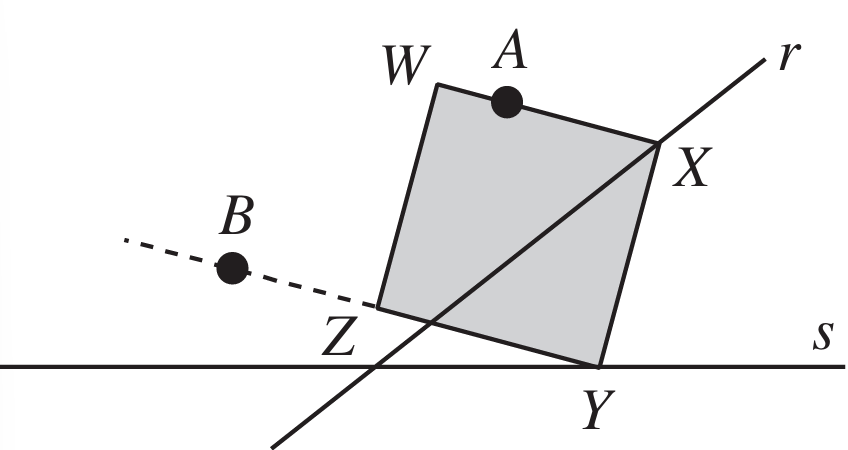
\includegraphics[width=0.4\textwidth]{images/kubična enačba/beloch_kvadrat.png}
    \caption[Belochin kvadrat]{Belochin kvadrat. Vzeto iz~\cite[str.\ 309]{hull2011}.}
    \label{fig:beloch_kvadrat}
\end{figure}

\opomba{V resnici nam v Belochinem postopku ne bo koristila konstrukcija samega kvadrata, pač pa bo dovolj le poiskati točki $X$ in $Y$. Skozinju bo namreč potekala želvina pot od točke $A$ do točke $B$, ki je po konstrukciji res sestavljena iz treh med seboj pravokotnih daljic.}
Belocheva pri postopku za konstrukcijo kvadrata navaja naslednje korake:
\begin{enumerate}
    \item Najprej konstruiramo premico $r'$, ki je vzporedna premici $r$ in od nje enako oddaljena kot točka $A$, tako da premica $r$ leži med točko $A$ in premico $r'$. Na enak način premici $s$ konstruiramo njeno vzporednico $s'$ (slika~\ref{fig:beloch_kvadrat_konstrukcija} levo).
    \item Opravimo Belochin pregib, ki točko $A$ slika v točko $A'$ na premici $r'$, točko $B$ pa v točko $B'$ na premici $s'$ (slika~\ref{fig:beloch_kvadrat_konstrukcija} na sredi).
    \item Naj bo točka $X$ središče daljice $AA'$ in točka $Y$ središče daljice $BB'$. Po konstrukciji novi točki sovpadata s presečiščem pregiba in premice $r$ oz.\ $s$. (slika~\ref{fig:beloch_kvadrat_konstrukcija} desno). Daljica $XY$ je pravokotna na daljici $AX$ in $BY$, zato samo še določimo točki $W$ in $Z$ na daljicah ali njunih nosilkah in tako dobimo Belochin kvadrat.
\end{enumerate}

\begin{figure}[h]
    \centering
    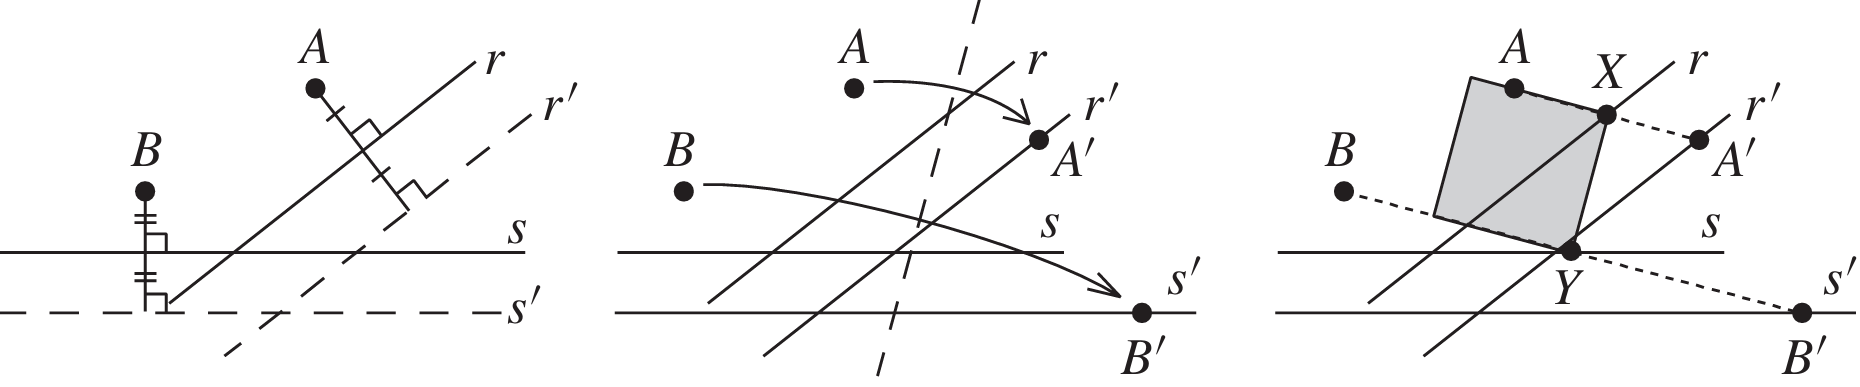
\includegraphics[width=0.95\textwidth]{images/kubična enačba/beloch_kvadrat_konstrukcija.png}
    \caption[Konstrukcija Belochinega kvadrata]{Konstrukcija Belochinega kvadrata z origamijem. Vzeto iz~\cite[str.\ 310]{hull2011}.}
    \label{fig:beloch_kvadrat_konstrukcija}
\end{figure}

\subsubsection*{Konstrukcija $\sqrt[3]{2}$ z Belochinim kvadratom}
\label{podpogl:beloch_kvadrat_koren}

Preden ravno naučeno znanje uporabimo za reševanje kubičnih enačb, si še na hitro poglejmo, kako lahko tudi z Belochinim kvadratom rešimo starogrški problem podvojitve kocke.

Za premico $r$ vzemimo ordinatno os, za premico $s$ pa abscisno os. Določimo še $A = (-1,0)$ in $B = (0, -2)$. Vzporednici sta torej $r': x = 1$ in $s': y = 2$. Belochin pregib seka premico $r$ v točki $X$, premico $s$ pa v točki $Y$ (slika~\ref{fig:beloch_koren}). Z $O$ označimo koordinatno izhodišče in opazimo podobne pravokotne trikotnike $OAX$, $OXY$ in $OYB$. Z upoštevanjem $|AO| = 1 $ in $|OB| = 2$ dobimo sledeča razmerja:
$$ \frac{|OX|}{|AO|} = \frac{|OY|}{|OX|} = \frac{|OB|}{|OY|} \Longrightarrow |OX| = \frac{|OY|}{|OX|} = \frac{2}{|OY|}, $$
iz česar sledi
$$ |OX|^3 = |OX| \cdot \frac{|OY|}{|OX|} \cdot \frac{2}{|OY|} = 2 \Longrightarrow |OX| = \sqrt[3]{2}. $$

\begin{figure}[h]
    \centering
    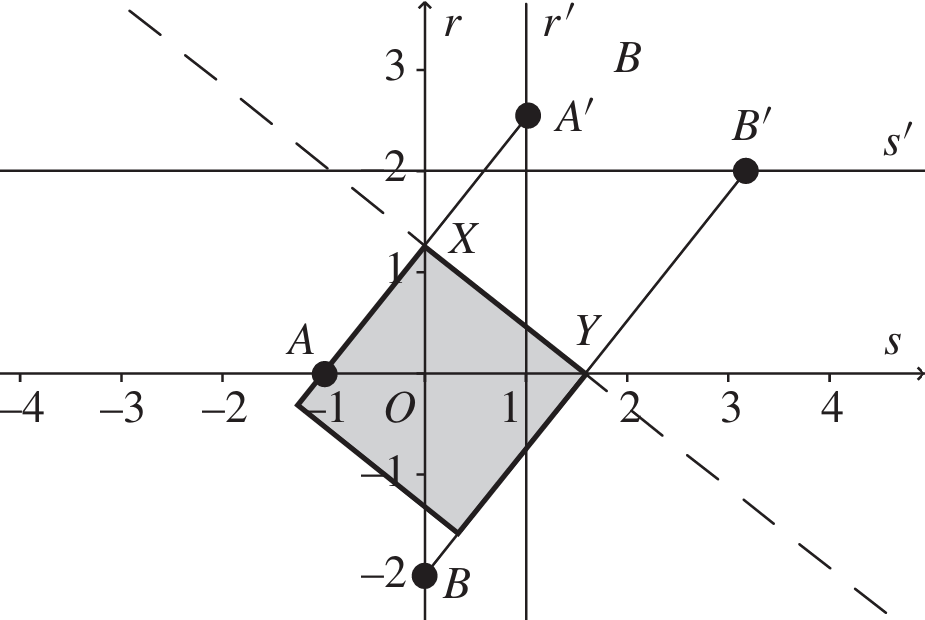
\includegraphics[width=0.5\textwidth]{images/kubična enačba/beloch_koren.png}
    \caption[Konstrukcija kubičnega korena števila dva]{Konstrukcija $\sqrt[3]{2}$ preko Belochinega kvadrata. Vzeto iz~\cite[str.\ 310]{hull2011}.}
    \label{fig:beloch_koren}
\end{figure}

Vidimo lahko, da je to enaka konstrukcija, kot jo je 50 let kasneje neodvisno od Belocheve odkril G.\ Martin (gl.\ razdelek~\ref{podpogl:podvojitev_kocke}), le da je za točko $B$ vzel točko $(0, -k)$ in s tem konstruiral dolžino $\sqrt[3]{k}$ za poljubno origami število $k$.

\subsubsection*{Združitev Lillove metode in Belochinega kvadrata v Belochin postopek}

Za poljubno enačbo $a x^3 + b x^2 + c x + d = 0$ povežimo sedaj Lillovo metodo s konstrukcijo primernega Belochinega kvadrata, ki nam bo natančno določil kot $\theta$. Belochin postopek, ki je opisan v nadaljevanju, velja za vsako izbiro koeficientov enačbe (gl.\ tudi sliko~\ref{fig:beloch_kubicna_resitev}):

\begin{enumerate}
    \item Za točko $A$ vzemimo izhodišče $O$. Začrtamo želvino pot za polinom $p(x) = a x^3 + b x^2 + c x + d$, ki se začne v točki $A$ in konča v točki $B$.
    \item Premica $r$ naj bo nosilka daljice $b$ ($r: x = a$), premica $s$ pa nosilka daljice $c$ ($s: y = b$).
    \item Določimo premici $r': x = 2a$ in $s': y = b + d$ ter opravimo Belochin pregib, ki točko $A$ položi na premico $r'$ in točko $B$ na premico $s'$.
    \item Presečišči pregiba s premicama $r$ in $s$ zaporedoma označimo s točkama $X$ in $Y$.
    \item Zarišemo daljice $AX$, $XY$ in $YB$.
\end{enumerate}

Ker po konstrukciji velja $ AX \perp XY \perp YB $, je to iskana pot laserskega žarka, ki se odbija pod pravim kotom in zadene želvo. Kot $\theta$ je kot, ki ga oklepata daljici $a$ in $AX$. Rešitev je torej $x_{\theta} = - \tan \theta$.

\begin{figure}[h]
    \centering
    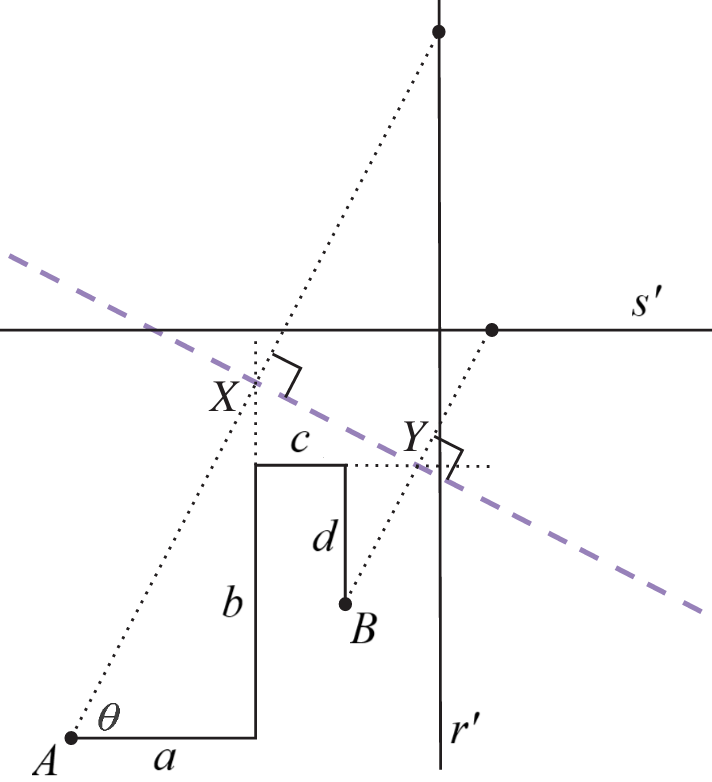
\includegraphics[width=0.4\textwidth]{images/kubična enačba/beloch_kubicna_resitev.png}
    \caption[Lillova metoda z Belochinim kvadratom]{Konstrukcija želvine poti za Lillovo metodo preko Belochinega kvadrata. Vzeto in preurejeno iz~\cite[str.\ 313]{hull2011}.}
    \label{fig:beloch_kubicna_resitev}
\end{figure}

\opomba{Če ima enačba še dve realni rešitvi, sta možna tudi še dva Belochina pregiba (enačba namreč ne more imeti točno dveh realnih rešitev, saj kompleksne rešitve nastopajo v konjugiranih parih).}

Kot zanimivost Lavričeva v~\cite[str.\ 10--13]{lavric2013} s postopkom, ki je malo preurejen Belochin postopek, še analitično pokaže, da je ob primerno izbranih točkah $A$ in $B$ ter premicah $r$ in $s$ koeficient premice, ki jo predstavlja Belochin pregib, rešitev kubične enačbe. Točki in premici izbere tako, da sta točki $X$ in $Y$ ravno presečišči z ordinatnima osema, iz česar lahko takoj razberemo koeficient premice. V dokazu izpelje enačbi pripadajočih parabol in splošno enačbo njunih tangent ter iz tega dokaže rečeno. To je lahko odlična vaja za dijake, ki si želijo dodatnega izziva.

\subsubsection*{Primer reševanja kubične enačbe z Belochinim postopkom}

Več primerov uporabe Belochinega postopka za reševanje kubičnih enačb je opisanih v~\cite[38--44]{zore2022}, tu pa si poglejmo, kako rešimo enačbo, ki ima tako pozitivne kot tudi negativne in ničelne koeficiente. Hull v~\cite[str.\ 90--92]{hull2013} obravnava enačbo
$$ x^3 - 7x - 6 = 0.$$
Po Lillovi metodi za točko $A$ vzamemo izhodišče $O$ in začrtamo želvino pot. Najprej gremo za $1$ v desno ($a=1$), se obrnemo za $90^\circ$ v pozitivno smer in obstojimo na mestu ($b=0$), se zopet obrnemo  $90^\circ$ v pozitivno smer in se premaknemo za $7$ v nasprotno smer, torej zopet v desno ($c=-7$), na koncu pa se po ponovnem obratu za $90^\circ$ v pozitivno smer premaknemo za 6 navzgor ($d=-6$). Končamo v točki $T = (8, 6)$.

Označimo še premice $r: x = a = 1, r': x = 2a = 2$ (na sliki~\ref{fig:lill_primer1} označena z $L_1$), $s: y = b = 0$ in $s': y = b + d = -6$ (na sliki~\ref{fig:lill_primer1} označena z $L_2$).

\begin{figure}[h]
    \centering
    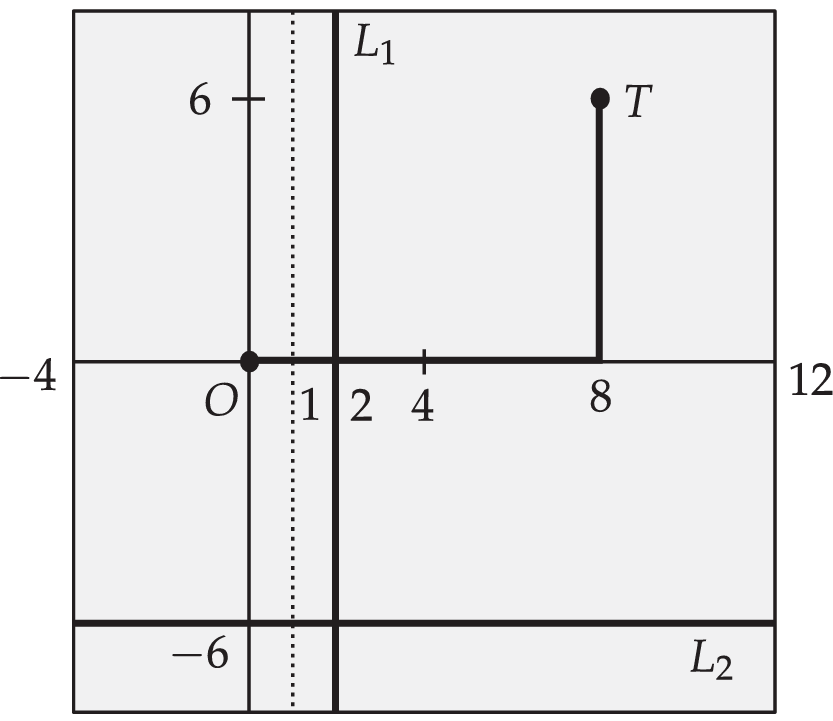
\includegraphics[width=0.4\textwidth]{images/kubična enačba/lill_primer_setup.png}
    \caption[Primer reševanja z Lillovo metodo (priprava)]{Priprava želvine poti in premic za reševanje enačbe z Lillovo metodo. Vzeto iz~\cite[str. 87]{hull2013}.}
    \label{fig:lill_primer1}
\end{figure}

Želvina pot je sedaj pripravljena, da točko $O$ prepognemo na premico $L_1$ in hkrati točko $T$ na premico $L_2$. Presečišči pregiba s premicama $r$ in $s$ nam data točki, kjer se laserski žarek za pravi kot odbije in na koncu zadane točko $T$. Kot, ki ga oklepa žarek z $x$-osjo ob koordinatnem izhodišču, nam podaja rešitev enačbe.

Na sliki~\ref{fig:lill_primer_pregibi} so konstrukcije vseh treh možnih pregibov. Začnimo z leve proti desni in za vsakega od njih pogledamo, kaj dobimo:
\begin{enumerate}
    \item V prvem primeru se nam točka $O$ preslika v točko $(2,2)$, točka $T$ pa v točko $(-4,-6)$, torej je kot $\theta = 45^\circ$, kar pomeni $x_{45^\circ} = -\tan 45^\circ = -1$. Preverimo, ali $x_{45^\circ}$ res reši našo enačbo. Zares, $(-1)^3 - 7\cdot(-1) - 6 = 0$.
    \item Točka $T$ se v drugem primeru preslika ravno v presečišče premic $L_1$ in $L_2$, torej v točko $(2,-6)$. Pregib torej premico $s$, ki je v našem primeru kar $x$-os, seka v točki $(5,0)$ (ker je presečišče središče daljice s krajišči v točki $T$ in njeni sliki). Rešitev $x_\theta$ lahko preberemo kar iz zadnjega pravokotnega trikotnika preko definicije kotne funkcije tangens: $x_\theta = -tan \theta = -6/3 = -2$. In res je $(-2)^3 - 7\cdot(-2) - 6 = 0$.
    \item V zadnjem primeru pa se v presečišče premic $L_1$ in $L_2$ preslika izhodišče $O$. Zato pregib premico $r$ seka v točki $(1,-3)$ in za kot $\theta$ gledamo prvi pravokotni trikotnik. Dobimo $x_\theta = -tan \theta = -(-3)/1 = 3$. Preverimo rešitev in dobimo $3^3 - 7\cdot3 - 6 = 0$.
\end{enumerate}

\begin{figure}[h]
    \centering
    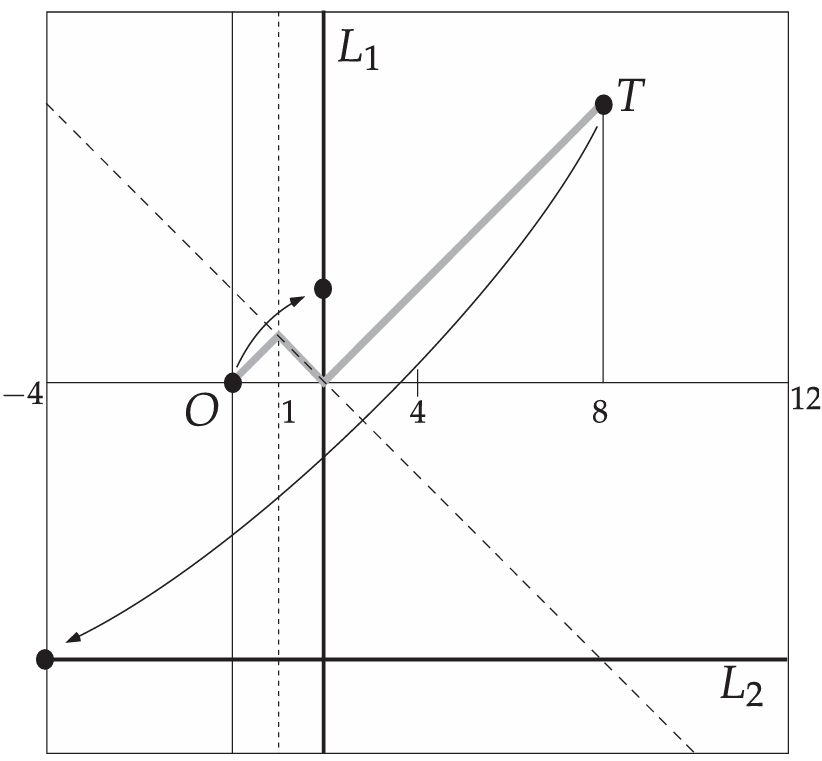
\includegraphics[width=0.33\textwidth]{images/kubična enačba/lill_primer_pregib1.png}
    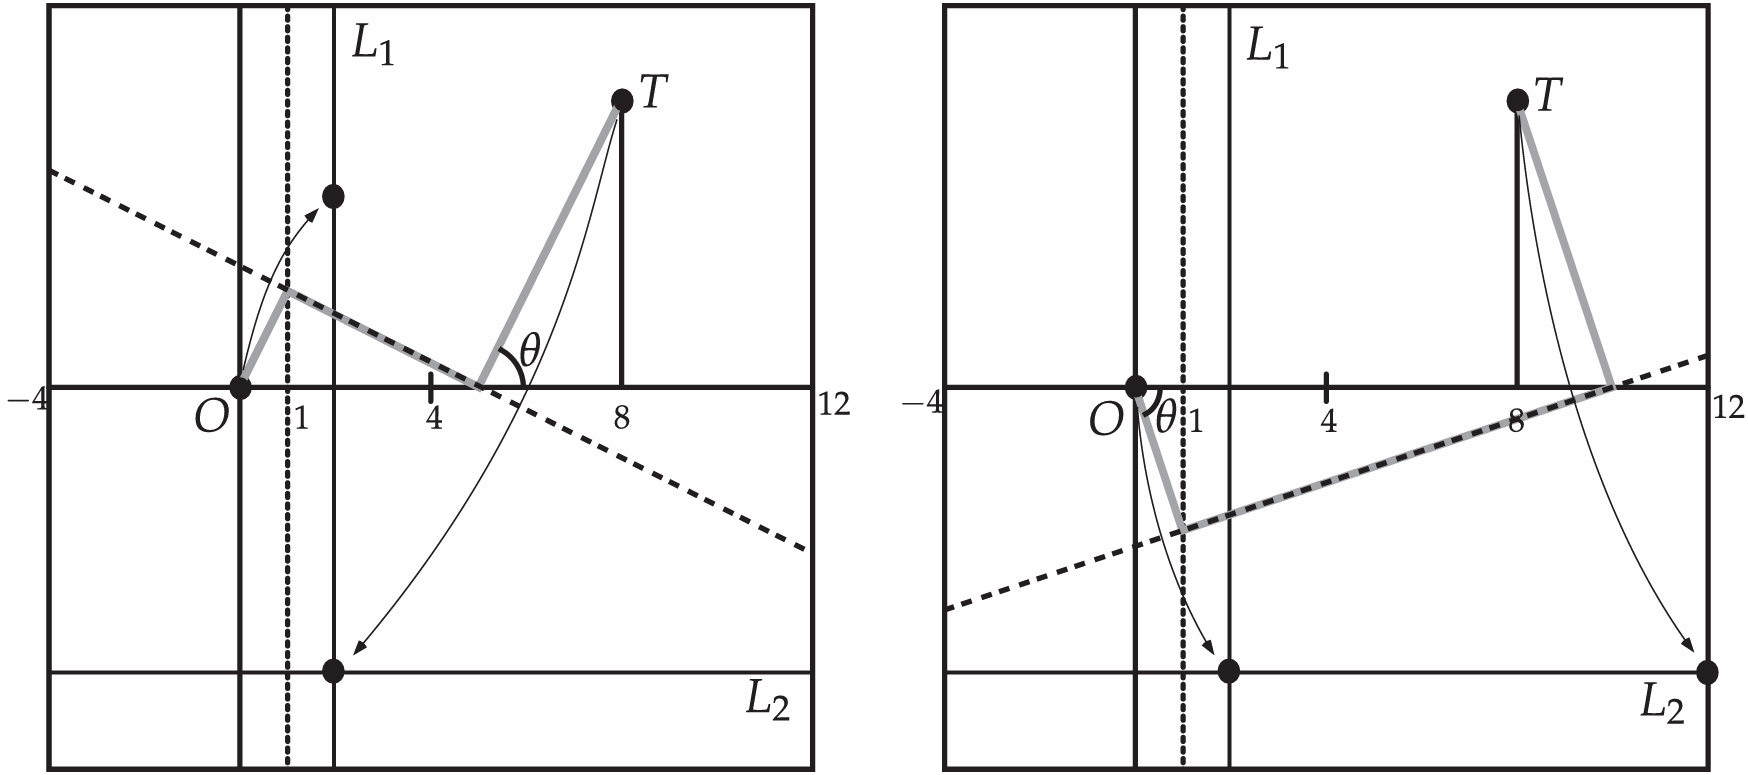
\includegraphics[width=0.65\textwidth]{images/kubična enačba/lill_primer_pregib2_3.png}
    \caption[Primer reševanja z Lillovo metodo (s pregibi)]{Pregibi, ki rešijo kubično enačbo $x^3 - 7x - 6 = 0$. Vzeto iz~\cite[str. 91--92]{hull2013}.}
    \label{fig:lill_primer_pregibi}
\end{figure}

Seveda se da enačbo $x^3 - 7x - 6 = 0$ hitreje rešiti z računanjem, vendar je ravno zaradi tega lep primer za uporabo Lillove metode z Belochinim pregibom, saj se da rešitve iz konstrukcije (ob natančnih prepogibih) takoj prebrati.

\subsubsection{Hatorijeva konstrukcija}

Japonski matematik Koshiro Hatori navaja postopek, ki je zelo podoben Belochinem postopku, vendar ga je avtor iznašel neodvisno od Belochinega dela in to kar pol stoletja za tem. Brez škode za splošnost predpostavi $a = 1$ in za reševanje enačbe $x^3 + bx^2 + cx + d = 0$ sledi naslednjim korakom (slika~\ref{fig:hatori}):
\begin{enumerate}
    \item V koordinatnem sistemu označimo točki $A = (b, 1)$ in $B = (d, c)$ ter premici $r': y = -1$ in $s': x = -d$.
    \item Opravimo pregib, ki točko $A$ položi na premico $r'$ ter točko $B$ na premico $s'$ (to je ravno Belochin pregib).
    \item Koeficient opravljenega pregiba je rešitev dane enačbe.
\end{enumerate}

\begin{figure}[h]
    \centering
    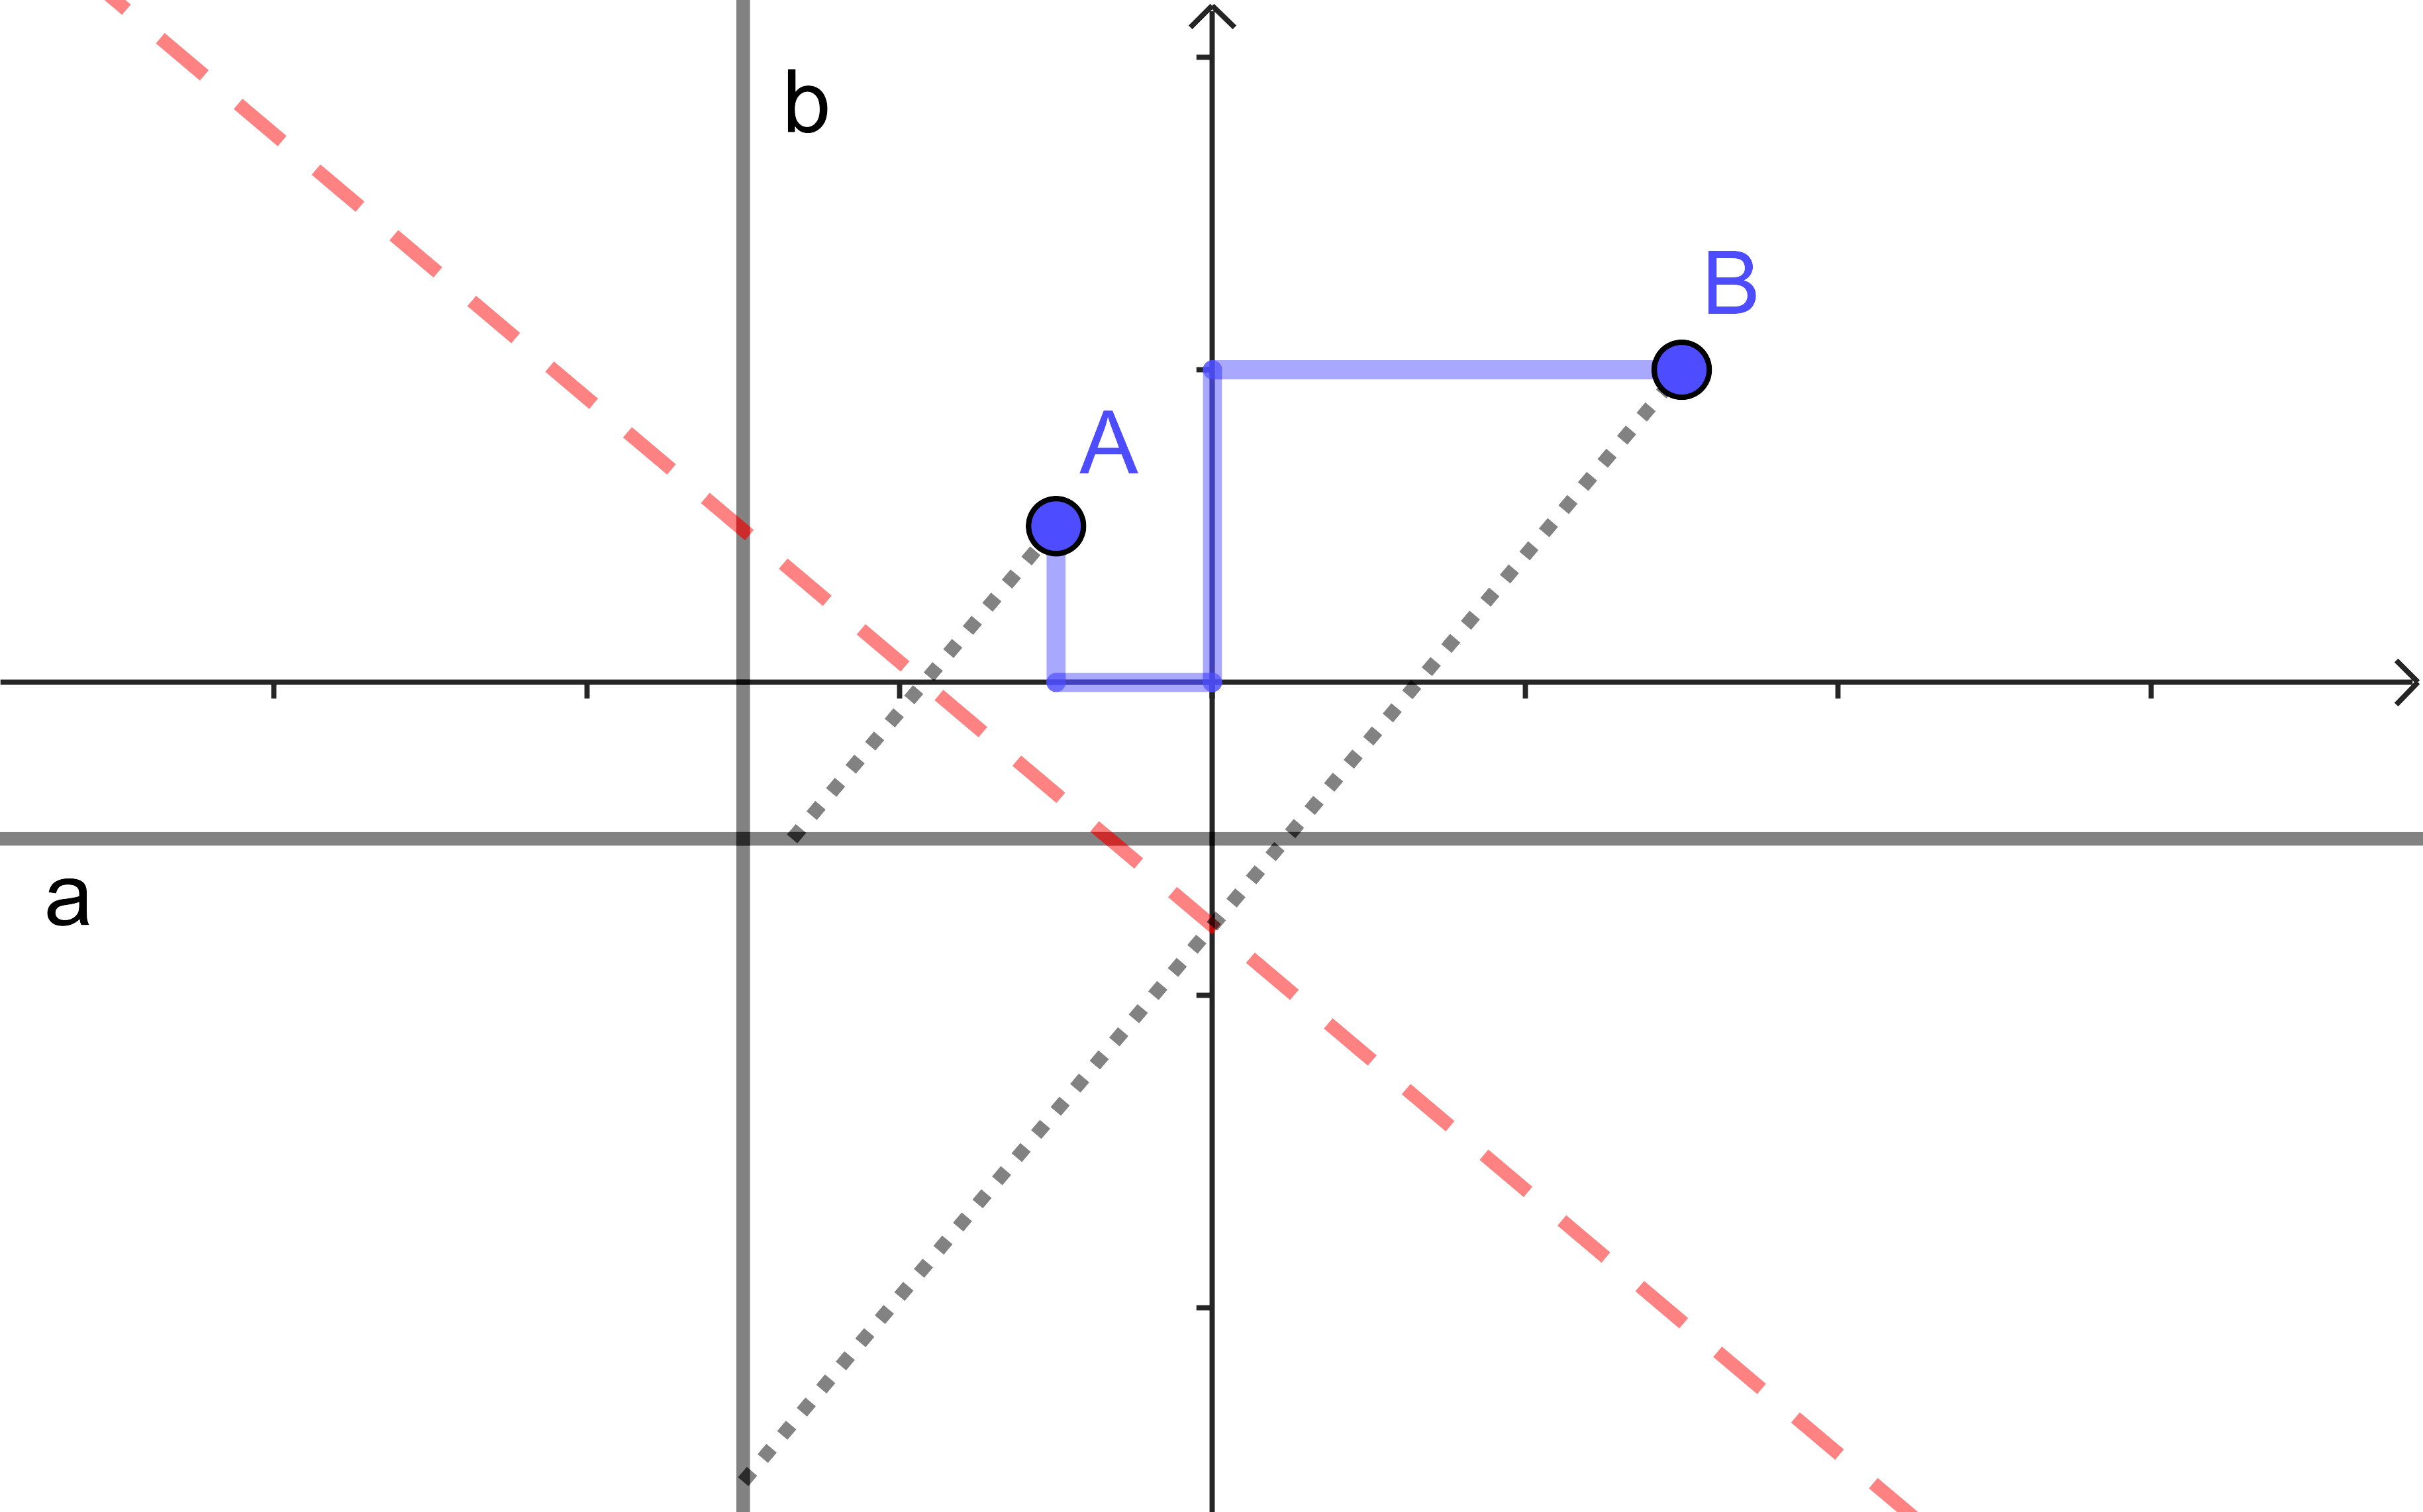
\includegraphics[width=0.5\textwidth]{images/kubična enačba/hatori.png}
    \caption[Hatorijeva konstrukcija]{Hatorijeva konstrukcija za enačbo $x^3 - x^2 + 2x + 3 = 0$.}
    \label{fig:hatori}
\end{figure}

Takoj vidimo, da je to v resnici ravno Belochin postopek, le da Hatori ne omeni premic $r$ in $s$ ter da se želva na začetku svoje poti ne nahaja v koordinatnem izhodišču temveč v točki $A$, je najprej usmerjena navzdol in se obrača v negativno smer (njena pot je na sliki~\ref{fig:hatori} označena z modro). Če izrazimo koeficient pregiba preko kota $\theta$, ki ga ob začetni točki $A$ omejujeta modra in črna prekinjena daljica, res dobimo $k = - \tan \theta$. Za geometrijsko razlago preko parabol gl.~\cite{hatori2003}.

\opomba{Seveda bi lahko vzeli katerikoli $a \in \Q$ in vzeli premico $r': y = -a$.}

\subsubsection{Reševanje kvadratne enačbe z Lillovo metodo}
\label{podpodl:kvadr_en_lill}

Lillovo metodo lahko uporabimo tudi za reševanje kvadratne enačbe $a x^2 + b x + c = 0$, kjer $a, b, c \in \Q$ in $a \neq 0$. Na enak način v koordinatni sistem zarišemo želvino pot, ki se začne v točki $A$ in konča v točki $B$. Za razliko od Belochinega postopka tu ne uporabimo Belochinega pregiba, temveč pregib iz operacije~\ref{op:O6}. Namesto dveh premic $r$ in $s$ imamo le eno -- naj bo $r$ nosilka daljice $b$. Kot prej -- na razdalji $a$ na drugi strani točke $A$ -- označimo še njeno vzporednico $r'$. Konstruiramo pregib, ki gre skozi točko $B$ in točko $A$ položi na premico $r'$. Njegovo presečišče s premico $r$ nam določi točko $X$, kjer se žarek iz točke $A$ pod pravim kotom odbije v točko $B$ (primer na sliki~\ref{fig:kv_en_lill}). S tem je kot $\theta$ določen. Vemo že, da sta možana največ dva pregiba in da je število pregibov enako številu realnih rešitev enačbe.

\begin{figure}[h]
    \centering
    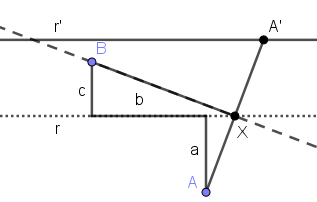
\includegraphics[width=0.4\textwidth]{images/kvadratna_enacba/kvadratna_enacba_lillova_metoda.png}
    \caption[Lillova metoda za kvadratno enačbo]{Reševanje kvadratne enačbe po Lillovi metodi z operacijo~\ref{op:O6} ($c < 0$).}
    \label{fig:kv_en_lill}
\end{figure}

\subsection{Alperinova in Geretschlägerjeva metoda za reševanje kubičnih enačb}
\label{podpogl:alperin}

V razdelku~\ref{podpogl:kvadratna_enacba} smo reševali kvadratno enačbo preko konstrukcije tangente na parabolo (operacija~\ref{op:O6}), ki je bila določena s koeficienti iz dane enačbe. Nato smo spoznali Belochin postopek, ki se poslužuje Belochinega pregiba (operacije~\ref{op:O7}), vendar brez povezave s parabolami. To povezavo bomo pogledali sedaj.

Alperin v~\cite[str.\ 129]{alperin2000} sicer namesto splošne kubične enačbe vzame zreducirano\footnote{V splošno kubično enačbo $x^3 + bx^2 + cx + d = 0$ vpeljemo novo spremenljivko $z = x - (1/3)b$. Bralec lahko za vajo izračuna, da s tem dobimo splošno kubično enačbo za $z$ brez kvadratnega člena.} obliko $x^3 + cx + d = 0$, kjer sta $c, d \in \Q$. Iz njenih koeficientov izbere naslednji paraboli:
\begin{itemize}
    \item $\mathcal{P}_1: \left(y - \frac{c}{2}\right)^2 = 2dx$ z goriščem v točki $(\frac{d}{2}, \frac{c}{2})$ in premico vodnico $x = -\frac{d}{2}$ in
    \item $\mathcal{P}_2:  x^2 = 2y$ z goriščem v točki $(0, \frac{1}{2})$ in premico vodnico $y = -\frac{1}{2}$.
\end{itemize}
Avtor nato opravi Belochin pregib, ki gorišče vsake parabole položi na njeno premico vodnico in tako konstruira skupno tangento. Ker sta paraboli pravokotni, je tak pregib en sam.
Sedaj pa se ne poslužimo uporabe matrik kot v zgornjem postopku, temveč analitično izrazimo koeficient skupne tangente. Naj bodo $k$ iskani koeficient, $(x_0, y_0)$ točka tangentnosti na prvi in $(x_1, y_1)$ točka tangentnosti na drugi paraboli. Iz enačbe prve parabole z implicitnim odvajanjem in upoštevanjem $dy/dx = k$ dobimo
$$ 2\left(y - \frac{c}{2}\right) \frac{dy}{dx} = 2d, \; \text{ torej } \; y_0 = \frac{d}{k} + \frac{c}{2} \; \text{ in } \; x_0 = \frac{\left(y_0 - \frac{c}{2}\right)^2}{2d} = \frac{d}{2k^2},$$
iz enačbe druge parabole pa
$$ 2x = 2\frac{dy}{dx}, \; \text{ torej } \; x_1 = k \; \text{ in } \; y_1 = \frac{k^2}{2}. $$
Ko koordinate vstavimo še v formulo za koeficient premice skozi dve točki, dobimo
$$ k = \frac{y_1 - y_0}{x_1 - x_0} = \frac{\frac{k^2}{2} - \frac{d}{k} - \frac{c}{2}}{k - \frac{d}{2k^2}}.
$$
Enačbo poenostavimo in res dobimo $k^3 + ck + d = 0$, torej je koeficient skupne tangente rešitev izvorne zreducirane kubične enačbe.

\begin{opomba}
    \label{opom:geret_metoda}
    Na enak način je do rešitve kubične enačbe še pred Alperinom prišel Robert Geretschläger (gl.\ ~\cite[368--369]{geret1995}). V članku pa za razliko od Alperina postopek posploši na reševanje splošne kubične enačbe oblike $x^3 + bx^2 + cx + d = 0$. Pri tem se izbiro parabole $\mathcal{P}_2$ ohrani, enačbo prve parabole $\mathcal{P}_1$ pa nastavi na $(y-c/2)^2 = 2d(x+b/2)$, torej dobimo gorišče v točki $(-b/2+d/2, c/2)$ in premico vodnico $x = -b/2-d/2$.
\end{opomba}

\subsection{Reševanje starogrških problemov preko reševanja enačb}

V razdelku~\ref{podpogl:starogrskiproblemi} smo si že pogledali več konstrukcij, ki z Belochinim pregibom rešijo problem podvojitve kocke in trisekcije kota. Poglejmo na problema še pod lučjo novega znanja reševanja enačb z origamijem

Pri podvojitvi kocke rešujemo enačbo $x^3 - 2 = 0$. Bralec je povabljen, da jo reši z Belochinim postopkom preko Lillove metode. V resnici smo to že storili v v razdelku, kjer smo spoznali Belochin kvadrat. Konstrukcija kubičnega korena števila $2$, ki smo jo takrat spoznali (gl.\ sliko~\ref{fig:beloch_koren}), je ravno konstrukcija po Belochinem postopku, le da je zrcaljena preko abscisne osi in premaknjena za enoto v levo.

Enačbo lahko rešimo tudi z Alperinovim postopkom ali katerokoli drugo metodo za reševanje kubičnih enačb, ki je omenjena v tem poglavju. Videli smo že veliko podobnih metod in ni nemogoče, da kakšni postopki izhajajo iz drugih.

Pri problemu trisekcije kota se spomnimo zveze $\cos 3\theta = 4 \cos^3 \theta - 3 \cos \theta$. Naj bo za dan kot $3\theta$ označena konstanta $k = \cos 3\theta$ (npr.\ za $3 \theta = 60^\circ$, ki se ga z evklidskim orodjem ne da tretjiniti, je $k = 1/2$), iščemo pa $x = \cos \theta$. Torej rešujemo enačbo $4x^3-3x-k=0$. Zopet lahko izberemo poljubno metodo; v~\cite[str.\ 370]{geret1995} je zapisana konstrukcija gorišč in premic vodnic za uporabo Geretschlägerjeve oz.\ Alperinove metodo.

\subsection{Kubična in kvartična enačba v projektivni ravnini}
\label{podpogl:afina_proj_enacbe}

Matematika Edwards in Shurman se v~\cite{edwards2001} ukvarjata z reševanjem enačb tretje in četrte stopnje preko iskanja skupnih tangent na določene stožnice, pri tem pa uporabljata princip Belochinega pregiba. Tematike se lotevata na celovit način z obravnavo splošnih enačb stožnic v projektivni ravnini.

Pri kubični enačbi iz njenih koeficientov določita gorišči in premici vodnici dveh parabol, rešitve enačbe pa so \emph{koeficienti} skupnih tangent. Tak postopek smo sicer spoznali že v razdelku~\ref{podpogl:alperin}, tu pa ga bomo pogledali pod malo drugačno lučjo.

Postopek za reševanje kvartične enačbe je podoben, vendar avtorja z njim rešita le kvartične enačbe v reducirani obliki. Iz njenih koeficientov določita parabolo in krožnico, rešitve pa so \emph{začetne vrednosti} skupnih tangent.

\subsubsection*{Konstrukcija skupne tangente na parabolo in krožnico}

Ker do sedaj poznamo le konstrukcijo skupne tangente na dve paraboli, je na mestu vprašanje, kako postopati v primeru, ko imamo namesto ene parabole krožnico. Postopek je v svojem bistvu zelo enostaven:
\begin{enumerate}
    \item Naj bosta dani parabola z znanima goriščem in premico vodnico ter krožnica z znanima središčem polmerom. Teh dveh stožnic ni potrebno risati, ker potrebujemo omenjene podatke.
    \item Zarišemo krožnico z istim središčem in dvakratnim polmerom.
    \item Po zgledu Belochinega pregiba gorišče prepognemo na premico in hkrati središče na rob ravnokar narisane krožnice.
\end{enumerate}

Po operaciji~\ref{op:O6} je pregib tangenten na dano parabolo, ker pa je po konstrukciji simetrala in pravokoten na polmer večje krožnice, je tangenten tudi na krožnico z originalnim polemrom. Na sliki~\ref{fig:tang_kroznica_par} sta desno prikazani dani parabola $\mathcal{P}$ in krožnica $\mathcal{C}$, levo pa konstrukcije iz danih podatkov -- gorišče $F'$, premica vodnica $D'$, središče $O$ ter krožnica $2\mathcal{C}$ z dvakrat večjim polmerom. Na obeh slikah so konsturirani vsi štirje pregibi oz. skupne tangente.

\begin{figure}[h]
    \centering
    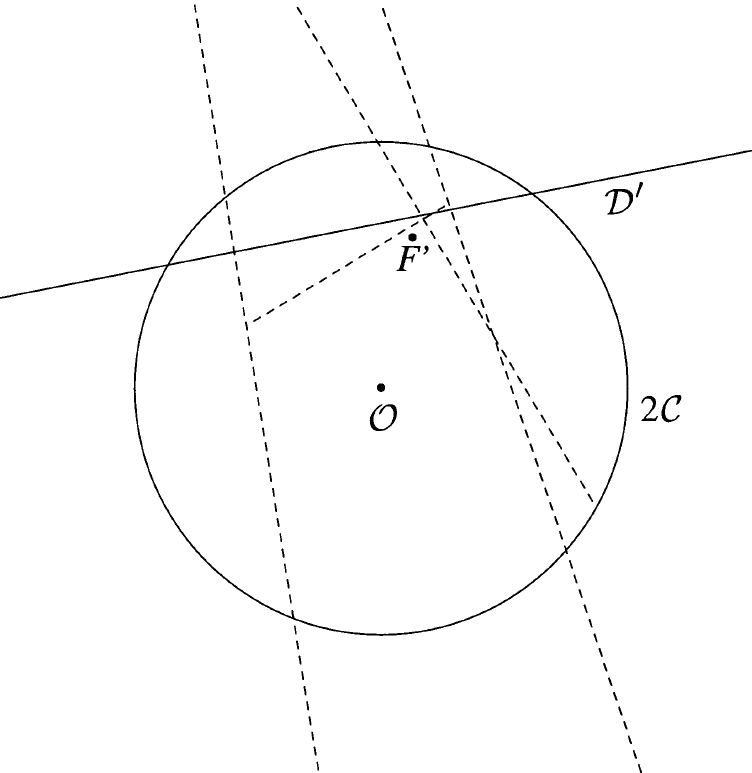
\includegraphics[width=0.48\textwidth]{images/tang_krozn_par1.png}
    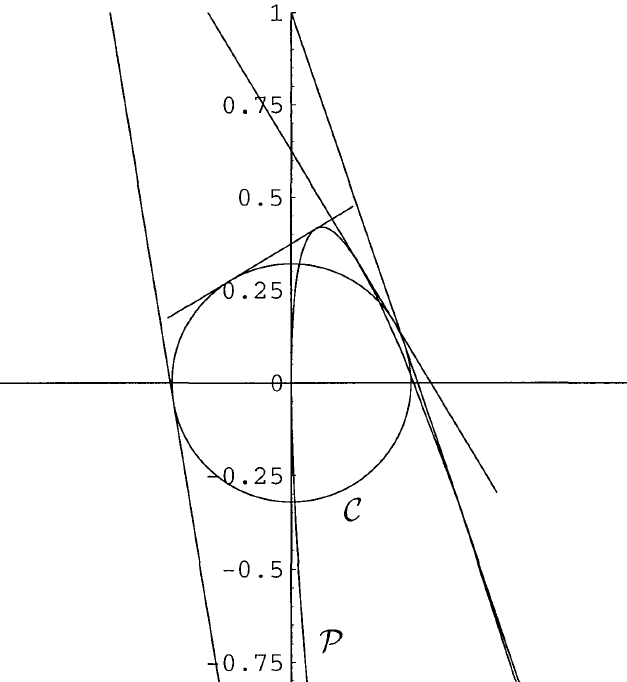
\includegraphics[width=0.5\textwidth]{images/tang_krozn_par2.png}
    \caption[Skupna tangenta na krožnico in parabolo]{Konstrukcija skupnih tangent na krožnico in parabolo. Vzeto iz~\cite[str.\ 24--25]{edwards2001}.}
    \label{fig:tang_kroznica_par}
\end{figure}

\begin{opomba}
    V tem razdelku za potrebe reševanja izjemoma potrebujemo šestilo, s katerim iz koeficientov kvartične enačbe konstruiramo krožnico.
\end{opomba}

Skupne tangente zato znamo zlahka konstruirati, pravo vprašanje pa je, kateri stožnici določa dana kubična oz.\ kvartična enačba. Kot omenjeno že v uvodu razdelka, si avtorja pri tem pomagata s projektivno ravnino. 

\subsubsection*{Stožnice v projektivni ravnini}

\textcolor{red}{Definicija projektivne geometrije nad vektorskim prostorom V (mi bomo imeli V = $\R^3$.)}

Stožnica $\mathcal{S}$ ima v $\mathcal{P}(\R^3)$ \textcolor{red}{(A ta``P'' je normalen font al tak kot tle?)} homogenizirano \textcolor{red}{(?)} enačbo
\begin{equation}
    \label{en:stoznica_splosna}
    \mathcal{S}: a_{11}x^2 + 2a_{12}xy + a_{22}y^2 + 2a_{13}xz + 2a_{23}yz + a_{33}z^2 = 0,
\end{equation}
kar lahko zapišemo v obliki
\begin{equation*}
    \mathcal{S}: v^\intercal M v = 0,
    \text{ kjer sta } v =
    \begin{bmatrix}
        x\\
        y\\
        z
    \end{bmatrix}
    \text{ in } M =
    \begin{bmatrix}
        a_{11} & a_{12} & a_{13}\\
        a_{12} & a_{22} & a_{23}\\
        a_{13} & a_{23} & a_{33}
    \end{bmatrix}.
\end{equation*}

Pri tem je simetrična matrika $M$ definirana do neničelnega skalarnega večkratnika natančno. Stožnica $\mathcal{S}$ je \emph{neizrojena} (ni unija dveh premic ali ene, dvojno štete premice), če ima poln rang, t.\ j.\ \textcolor{red}{rang (-- dej v matematično okolje?)} $ M = 3$ oz. ekvivalentno, $\det M \neq 0$. V nadaljevanju bomo delali le z neizrojenimi stožnicami, torej vedno obstaja inverz matrike $M$, ki je prav tako simetričen.

Iz prvega minorja matrike $M$ lahko takoj preberemo, za katero vrsto neizrojene stožnice gre. Naj bo $A_M = a_{11}a_{22} - a_{12}^2$ \textcolor{red}{(Vir tega je Wikipedia: Matrix representation of conic sections. Kakšen bolj zanesljiv vir?)}:
\begin{itemize}
    \item $\mathcal{S}$ je hiperbola, če in samo če $A_M < 0$,
    \item $\mathcal{S}$ je parabola, če in samo če $A_M = 0$ in
    \item $\mathcal{S}$ je elipsa, če in samo če $A_M > 0$. Če poleg tega velja še $a_{11} = a_{22}$ in $a_{12} = 0$, je $\mathcal{S}$ krožnica.
\end{itemize}

\textcolor{red}{(Definicija dualnosti?)}

\textcolor{red}{\emph{Dualno stožnico} (a je prevod ok?)} stožnice $\mathcal{S}$ definiramo z inverzno matriko:
\begin{equation*}
    \mathcal{\hat{S}}: v^\intercal M^{-1} v = 0.
\end{equation*}

Naj bo $p \in \mathcal{S}$ točka na stožnici $\mathcal{S}$ in naj bo $q = Mp$. Potem je
 $$q^\intercal M^{-1} q = (Mp)^\intercal M^{-1} (Mp) = p^\intercal M^\intercal M^{-1} M p = p^\intercal M p = 0,$$
 kar pomeni, da je $q \in \mathcal{\hat{S}}$. Ker je $M$ obrnljiva, je preslikava $\mathcal{S} \longrightarrow \mathcal{\hat{S}}$ s predpisom $p \mapsto Mp$ bijekcija med stožnico $\mathcal{S}$ in njeno dualno stožnico $\mathcal{\hat{S}}$. Kaj pa so točke dualne stožnice $\mathcal{\hat{S}}$? (\textcolor{red}{Dokončaj; zakaj je $q$ ravno tangenta na $\mathcal{S}$?})

 Naj bosta $\mathcal{S}_1$ in $\mathcal{S}_2$ stožnici s pripadajočima simetričnima obrnljivima matrikama $M_1$ in $M_2$. Potem je njuna skupna tangenta skupna točka njunih dualnih stožnic $\mathcal{\hat{S}}_1$ in $\mathcal{\hat{S}}_2$. Torej iščemo $q \in \mathcal{\hat{S}}_1, \mathcal{\hat{S}}_2$, (\textcolor{red}{a je q res prou tangenta? to je pač točka od dualne stožnice}) ki reši sistem enačb
 \begin{equation}
    \label{eq:afin_sistem_tangenta_splosen}
    q^\intercal M^{-1}_1 q = 0 \; \text{ in } \; q^\intercal M^{-1}_2 q = 0.
 \end{equation}
 \textcolor{red}{kakšne oblike je q? oziroma tangenta?}

 \subsubsection*{Reševanje kubične enačbe}

 Zopet rešujemo kubično enačbo oblike $ x^3 + bx^2 + cx + d = 0, d \neq 0$. Za stožnici vzamemo naslednji paraboli:
 \begin{itemize}
    \item $\mathcal{P}_1: (y+c)^2 = -4d(x-b)$ z goriščem $F_1 (b - d, -c)$ in premico vodnico $L_1: x = b + d$,
    \item $\mathcal{P}_2: x^2 = -4y$ z goriščem $F_2 (0, -1)$ in premico vodnico $L_2: y = 1$.
 \end{itemize}

 \opomba{Opazimo, da gre za enako izbiro parabol kot pri Geretschlägerjevi metodi (opomba~\ref{opom:geret_metoda}), le da so tu spremenljivke pomnožene za faktor $-2$.}

 Iz enačb parabol zapišemo njuni matriki
$$ M_1 =
    \begin{bmatrix}
        0 & 0 & 2d\\
        0 & 1 & c\\
        2d & c & c^2-4bd
    \end{bmatrix}
    \; \text{ in } \; M_2 =
    \begin{bmatrix}
        1 & 0 & 0\\
        0 & 0 & 2\\
        0 & 2 & 0
    \end{bmatrix}
$$
ter izračunamo njuna inverza
$$ M^{-1}_1 = \frac{1}{d}
    \begin{bmatrix}
        b & -c/2 & 1/2\\
        -c/2 & d & 0\\
        1/2 & 0 & 0
    \end{bmatrix}
\; \text{ in } \; M^{-1}_2 =
    \begin{bmatrix}
        1 & 0 & 0\\
        0 & 0 & 1/2\\
        0 & 1/2 & 0
    \end{bmatrix}.
$$

Naj bo $q = [A\;B\; C]^\intercal \in \mathcal{\hat{P}}_1, \mathcal{\hat{P}}_2$ skupna tangenta (\textcolor{red}{je to res ``tangenta'' al kako se temu reče?}) na paraboli $\mathcal{P}_1$ in $\mathcal{P}_2$. Iz sistema enačb~\ref{eq:afin_sistem_tangenta_splosen} dobimo nov sistem
\begin{equation}
    \label{eq:afin_sistem_tangenta_ABC_kub}
    bA^2 - cAB + AC + dB^2 = 0 \; \text{ in } \; -BC = A^2.
\end{equation}

Da dobimo \textcolor{red}{nevertikalno afino skupno} tangento na paraboli $\mathcal{P}_1$ in $\mathcal{P}_2$, normaliziramo $B = -1$ in $z = 1$, s čimer dehomogeniziramo (\textcolor{red}{? poglej kako je z izrazi, pa $z = 1$ je verjetno pač k je afina ravnina, zakaj pa je $B = -1$?}) tangento $Ax + By + Cz = 0$ v $y = Ax + C$. S tem se druga enačba v sistemu~\ref{eq:afin_sistem_tangenta_ABC_kub} preuredi v $C = A^2$, prva pa v
$$ A^3 + bA^2 + cA + d = 0,$$
kar pomeni, da nam $A$, koeficient skupne tangente, reši izvorno kubično enačbo.
\begin{opomba}
    S konstrukcijo pregibov pa še ne dobimo njegovega koeficienta. V praksi lahko to storimo tako, da poiščemo presečišče pregiba z $x$-osjo, npr.\ točko $(x_0, 0)$ in na razdalji $1$ v desno konstruiramo  pravokotnico na $x$-os skozi točko $(x_0 + 1, 0)$, ki bo tangento sekala ravno v točki $(x_0 + 1, A)$. Sedaj lahko tudi uradno potrdimo konstrukcijo realne rešitve kubične enačbe.
    \textcolor{red}{Lahko daš eno slikco za izi prikaz.} 
\end{opomba}

\textcolor{red}{Dodaj konkreten primer iz članka, origami pregibe si tudi fizično sprobala na enem listi.}

\subsubsection*{Reševanje kvartične enačbe}

Kot že povedano, sledeči postopek ne rešuje splošne enačbe četrte stopnje, temveč njeno zreducirano obliko
\begin{equation}
    \label{eq:reduc_kvart_ev}
    x^4 + bx^2 + 2cx + d = 0
\end{equation}
(\textcolor{red}{Omeni, da se da vsako kvartično enačbo zreducirat v to?})
Smiselno predpostavimo $d \neq 0$, saj bi se v nasprotnem primeru pri eliminaciji ničle $x = 0$ enačba prevedla na kubično. Poleg tega predpostavimo še $c \neq 0$, ki nam prepreči, da bi se enačba z uvedbo nove spremenljivke za $x^2$ prevedla celo na kvadratno enačbo.

\textcolor{red}{omeni Bezuatov izrek al kaj je že in da dualne stožnice imajo kvadratno enačbo, kar pomeni, da imata dve največ štiri skupne točke (tangente) v kompleksni projektivni ravnini; ker so inverzne matrike realne, nastopajo v konjugiranih parih, torej imata po nič, dve ali štiri skupne tangente (šteto z večkratnostjo). A je tu not tudi tangenta v neskončnosti všteta? Skratka, dve paraboli pa imata skupno tangento v neskončnosti, kar pomeni, da potem ne pustita dovolj afinih tangent, ki bi rešile kvartično enačbo (ker so afine tangente največ tri). Zato ne moremo vzeti dveh parabol.}

Zgornjo metodo bi lahko uporabili tudi tu. Avtorja pri predpostavki $bd - c^2 \neq 0$ vzameta naslednji stožnici:
\begin{itemize}
    \item $\mathcal{S}: dx^2 + 2cxy + by^2 + bd - c^2 = 0$ in
    \item parabolo od prej, t.\ j.\ $\mathcal{P}: x^2 = -4y$.
\end{itemize}
Bralec je povabljen, da po enakem postopku kot pri kubični enačbi izpelje, da koeficient skupne tangente $y = Ax + C$ reši enačbo~\ref{eq:reduc_kvart_ev}. \textcolor{red}{(To si izpeljala)}. Stožnicama $\mathcal{S}$ in $\mathcal{P}$ zaporedoma pripadata matriki
$$ M_\mathcal{S} =
    \begin{bmatrix}
        d & c & 0\\
        c & b & 0\\
        0 & 0 & bd - c^2
    \end{bmatrix}
    \; \text{ in } \; M_\mathcal{P} =
    \begin{bmatrix}
        1 & 0 & 0\\
        0 & 0 & 2\\
        0 & 2 & 0
    \end{bmatrix}.
$$
Ker za glavni minor matrike $M_\mathcal{S}$ velja $A_{M_\mathcal{S}} = bd - c^2 \neq 0$, stožnica $\mathcal{S}$ ni parabola in ker velja $c \neq 0$, ne more biti niti krožnica. Torej je lahko le elipsa ali hiperbola. Tu pa nastane težava, saj avtorja nista uspela najti splošne geometrijske metode za konstrukcijo skupne tangente na parabolo in elipso oz.\ hiperbolo. Ker pa znamo konstruirati skupno tangento na parabolo in krožnico, predlagata malo prilagojen postopek, ki je sicer algebraično manj eleganten, vendar geometrijsko toliko lažje izveden.

Pri danih koeficientih $b, c, d$ enačbe~\ref{eq:reduc_kvart_ev} vpeljimo novi oznaki
$$ e = \frac{\sqrt{bd - c^2}}{d} \; \text{ in } \; r = |e|\sqrt{-d}, $$
iz česar sledita relaciji, ki ju bomo kasneje uporabili pri izpeljavi:
\begin{equation}
    \label{eq:kvarticni_relaciji}
    b= de^2 + \frac{c^2}{d^2} \; \text{ in } \; -\frac{de^2}{r^2} = 1.
\end{equation}
\opomba{Smiselno za koeficiente $b, c, d$ predpostavimo $bd - c^2 > 0$ in $d < 0$. Zato s tem postopkom ne moremo reševati poljubnih enačb četrte stopnje.}
Avtorja nato predlagata naslednji matriki za dualni stožnici $\mathcal{\hat{C}}$ in $\mathcal{\hat{P}}$:
$$ M^{-1}_\mathcal{C} =
    \begin{bmatrix}
        1 & 0 & 0\\
        0 & 1 & 0\\
        0 & 0 & -1/r^2
    \end{bmatrix}
\; \text{ in } \; M^{-1}_\mathcal{P} =
    \begin{bmatrix}
        0 & 0 & de/2\\
        0 & -d & c/2\\
        de/2 & c/2 & 0
    \end{bmatrix}.
$$
Če izračunamo njuna inverza, dobimo matriki
$$ M_\mathcal{C} =
    \begin{bmatrix}
        1 & 0 & 0\\
        0 & 1 & 0\\
        0 & 0 & -r^2
    \end{bmatrix}
    \; \text{ in } \; M_\mathcal{P} = -\frac{1}{d^3e^2}
    \begin{bmatrix}
        c^2 & -cde & -2d^2e\\
        -cde & d^2e^2 & 0\\
        -2d^2e & 0 & 0
    \end{bmatrix}.
$$
Iz njiju zapišemo predpisa stožnic v afini ravnini ($z = 1$) in dobimo:
\begin{itemize}
    \item krožnico $\mathcal{C}: x^2 + y^2 = r^2$ s središčem v $S(0,0)$ in polmerom $r$ ter
    \item parabolo $\mathcal{P}: c^2x^2 - 2cdexy + d^2e^2y^2 - 4d^2ex = 0$ (ker je $A_{M_\mathcal{P}} = 0$, je $\mathcal{P}$ res parabola).
\end{itemize}
Z določitvijo gorišča in premice vodnice parabole $\mathcal{P}$ se bomo ukvarjali pozneje; najprej algebraično poiščimo skupno tangento na dani stožnici.

Naj bo $q = [A\;B\; C]^\intercal$ presečišče dualnih stožnic $\mathcal{\hat{C}}$ in $\mathcal{\hat{P}}$. Iz sistema enačb~\ref{eq:afin_sistem_tangenta_splosen} dobimo nov sistem
\begin{equation}
    \label{eq:afin_sistem_tangenta_ABC_kvart}
    A^2 + B^2 = \frac{C^2}{r^2} \; \text{ in } \; deAC - dB^2 + cBC = 0.
\end{equation}
Z določitvijo $B = -1$ in $z = 1$ zopet dobimo afino obliko skupne tangente kot $y = Ax + C$. Ko $B$ vstavimo v sistem~\ref{eq:afin_sistem_tangenta_ABC_kvart}, prvo enačbo množimo z $de^2C^2$, drugo kvadriramo, delimo z $d$ in vstavimo v prvo enačbo, dobimo
$$ - \frac{de^2}{r^2}C^4 - (de^2 + \frac{c^2}{d})C^2 + 2cC + d = 0.$$
V dobljeno enačbo vstavimo relaciji~\ref{eq:kvarticni_relaciji} in dobimo
$$C^4 + bC^2 + 2cC + d = 0,$$
kar pomeni, da nam $C$, začetna vrednost tangente oz.\ njeno presečišče z ordinatno osjo reši izvorno kvartično enačbo.

Sedaj poiščimo še gorišče in premico vodnico parabole $\mathcal{P}$. Potem bo postopek konstrukcije skupne tangente, kot smo ga opisali že zgoraj -- najprej narišemo krožnico s središčem $S$ in polmerom $2r$ ter gorišče in premico vodnico parabole. Nato opravimo pregib, ki hkrati položi gorišče na premico vodnico in središče krožnice na njen rob. Presečišče pregiba z ordinatno osjo je rešitev naše enačbe (seveda poiščemo vse možne pregibe, ki so največ štirje).

Iz enačbe parabole $\mathcal{P}: c^2x^2 - 2cdexy + d^2e^2y^2 - 4d^2ex = 0$ ne moremo enostavno prebrati gorišča in premice vodnice, zato $(x, y)$-sistem prevedimo v \textcolor{red}{(a je izraz primeren?)} $(z, w)$-sistem s sledečo preslikavo \textcolor{red}{(od kje pride ta $P$?)}:
$$ \begin{bmatrix} x\\y\\1\end{bmatrix} = P \cdot \begin{bmatrix} z\\w\\1\end{bmatrix}, \text{ kjer je } P =
\begin{bmatrix}
    c/bd & de & c^2e/b^2\\
    -e/b & c & -(bc + cde^2)/b^2\\
    0 & 0 & 1
\end{bmatrix}.
$$

Ko to vstavimo v matrično enačbo parabole $[x\;y\;1] P [x\;y\;1]^\intercal$, po računanju in poenostavljanju\footnote{Za izračun je potrebna programska oprema, kot je npr.\ Wolfram Mathematica. \textcolor{red}{imaš zračunano, lahko vstavim tle screenshot za dokaz, da sem zračunala?}} na koncu dobimo
$$ \mathcal{P}: z^2 = 4d^3e^2w. $$

V $(z, w)$ sistemu ima parabola gorišče v $F_{zw}(0, d^3e^2)$ in premico vodnico $L_{zw}: w = - d^3e^2$ oziroma $L_{zw}: (z, w) = (0, -d^3e^2) + t(1, 0), t \in \R $. Izhodišče v $(x, y)$-sistemu je tako v točki $O_{xy} (c^2e/b^2, -(bc + cde^2)/b^2)$. Iz tega lahko izračunamo še gorišče in premico vodnico v $(x, y)$-sistemu:
$$ F_{xy} = P \cdot \begin{bmatrix} 0\\d^3e^2\\1\end{bmatrix} \longrightarrow F_{xy} = O_{xy} + d^3e^2(de, c) = (\frac{c^2e}{b^2} + d^4e^3, -\frac{bc + cde^2}{b^2} + cd^3e^2),$$
$$ L_{xy} = P \cdot \left( \begin{bmatrix} 0\\-d^3e^2\\1\end{bmatrix} + t \cdot \begin{bmatrix} 1\\0\\1\end{bmatrix} \right) \longrightarrow L_{xy}: (x, y) = O_{xy} - d^3e^2(de, c) + t(c, -de), t \in R.$$

V eksplicitni obliki je enačba za premico vodnico
$$ L_{xy}: y = -\frac{de}{c} \cdot x - \frac{1}{bc} (c^2 + bc^2d^3e^2 + bd^5e^4). $$

Kot vidimo, gorišče in premica vodnica nimata lepih predpisov, vendar je po eni strani ta metoda precej bolj zanimiva kot pretvorba kvartične enačbe na enačbe nižje stopnje in reševanje z običajno Lillovo metodo.

\textcolor{red}{lahko daš še slikovni primer (slika 4 iz istega vira) poleg konkretne enačbe, samo za okus. Sta pa slika 3 in slika 4 povezani med sabo, gre za iste podatke.}